\documentclass{sig-alternate-05-2015}
%\paperwidth=8.5in
%\paperheight=11in
%\usepackage[margin=1in]{geometry}

\usepackage{amsmath,amsfonts,amssymb}
\usepackage{color}
\usepackage{graphicx}
\usepackage{epsfig}
\usepackage{url}
\usepackage{semantic}
\usepackage{subfigure}
\newcommand{\figref}[1]{Figure \ref{#1}}
\newcommand{\tabref}[1]{Table \ref{#1}}
\newcommand{\eqnref}[1]{Equation \ref{#1}}
\newcommand{\KZ}[1]{\textcolor{blue}{(KZ: #1)}}
\newcommand{\ZY}[1]{\textcolor{red}{(#1)}}
\newcommand{\ERIC}[1]{\textcolor{green}{(Eric: #1)}}
\newcommand{\cut}[1]{}
\newcommand{\dd}[0]{\mathrm{d}}
\newcommand{\numberthis}{\stepcounter{equation}\tag{\theequation}}

\usepackage{courier}
\usepackage{listings}
\lstset{ %
	numberstyle=\scriptsize,
	basicstyle=\scriptsize\ttfamily,
	breaklines=true,
	tabsize=1,
	columns=fullflexible,
	numbers=left,
	stepnumber=1
}

\usepackage{etoolbox}
\makeatletter
\patchcmd{\maketitle}{\@copyrightspace}{}{}{}
\makeatother

\DeclareMathOperator*{\var}{var}
\DeclareMathOperator*{\val}{val}
\DeclareMathOperator*{\dom}{dom}

\mathlig{=>}{\Rightarrow}
\mathlig{->}{\rightarrow}

\newcounter{enum}
\newenvironment{packed_enum}{
%\begin{list}{\arabic{enum}.}{
\begin{list}{(\alph{enum})}{
  \setlength{\itemsep}{-0.5pt}
  \setlength{\parskip}{1pt}
  \setlength{\labelwidth}{30 pt}
  \setlength{\leftmargin}{15 pt}
  \setlength{\itemindent}{0pt}
  \usecounter{enum}}
}{\end{list}}


\makeatletter
\newcommand{\Spvek}[2][r]{%
  \gdef\@VORNE{1}
  \left(\hskip-\arraycolsep%
    \begin{array}{#1}\vekSp@lten{#2}\end{array}%
  \hskip-\arraycolsep\right)}

\def\vekSp@lten#1{\xvekSp@lten#1;vekL@stLine;}
\def\vekL@stLine{vekL@stLine}
\def\xvekSp@lten#1;{\def\temp{#1}%
  \ifx\temp\vekL@stLine
  \else
    \ifnum\@VORNE=1\gdef\@VORNE{0}
    \else\@arraycr\fi%
    #1%
    \expandafter\xvekSp@lten
  \fi}
\makeatother

\newcommand\Mark[1]{\textsuperscript{#1}}

\begin{document}
%\pagestyle{empty}

\title{InferSpark: Statistical Inference at Scale}

%\numberofauthors{5}
\author{
Zhuoyue Zhao~\Mark{1}, Jialing Pei~\Mark{1}, Eric Lo~\Mark{2}, Kenny Q. Zhu~\Mark{1}, Chris Liu~\Mark{2}\\
\affaddr{\Mark{1}Shanghai Jiao Tong University \hspace*{4mm}\Mark{2}Hong Kong Polytechnic University}\\
\email{
\{zzy7896321@, peijialing@, kzhu@cs\}.sjtu.edu.cn
\hspace*{2mm}\{ericlo, cscyliu\}@comp.polyu.edu.hk
}
}

\maketitle

%\unitlength1pt
%\begin{picture}(0,0)
%\put(380,190){\mbox{\Large \bf  Paper \#478}}
%\end{picture}
%\unitlength1cm


\begin{abstract}
%\KZ{
The Apache Spark stack has enabled fast
large-scale data processing.
Despite a rich library of statistical models and
inference algorithms, it does not give domain
users the ability to develop their own models.
%}
The emergence of probabilistic programming languages 
has showed the promise of developing sophisticated
probabilistic models in a succinct and programmatic way.
%helps data analysts and machine learning experts to concisely 
%describe the probabilistic models using a programming language. 
These frameworks have the potential of automatically generating
inference algorithms for the user defined models and 
answering various statistical queries about the model. 
It is a perfect time to unite these two great directions to
produce a programmable big data analysis framework. 
We thus propose, InferSpark, a probabilistic programming framework on top of Apache Spark. 
Efficient statistical inference can be easily implemented on this 
framework and inference process can leverage the distributed main memory processing 
power of Spark. This framework makes statistical inference on
big data possible and speed up the penetration of probabilistic 
programming into the data engineering domain. 
\end{abstract}

\section{Introduction}

Protein$-$protein interactions (PPIs) are of central importance for the majority of biological functions, such as signal transduction, metabolic pathways, molecular dynamics, and protein networks\cite{Hoffmann.Krallinger.ea:2005}, for they serve as the most fundamental building blocks of the entire interacademic systems of any organisms. Collecting data on pairwise interaction relationships is essential for multiple purpose, including identification of modules with certain functionality\cite{Spirin.Mirny.03}, mapping diseases to dominated genes\cite{Ideker.Sharan.08}, and after all, understanding wholistic metabolic/genetic networks from a system biology perspective.

A lot of databases have been built to store protein and genetic interactions from major model organism species and are available in various standardized formats, such as MINT\cite{Zanzoni.Montecchi-Palazzi.ea:2002}, BIND\cite{Bader.ea:2003}, BIOGRID\cite{DBLP:journals/nar/StarkBRBBT06}, etc. Among those mainstream databases, the data largely rely on voluntary reports by scientists or researchers, besides, comprehensive curation efforts become indispensable for the sake of accuracy. However, the amount of biology-related literatures with respect to protein interactions grows explosively and thus make it either impossible or impractical to manually detect PPI information anymore.

Considering huge amount of PPI information with great wealth hidden in published papers, in recent years, numerous mining techniques have been proposed that aim to extract PPI information automatically from free text, especially machine learning, information retrieval, and natural language processing\cite{DBLP:journals/bib/WinnenburgWPDS08}.These approaches can be roughly categorized into three classes: co$-$occurrence, rule$-$based, and machine learning. 

Co$-$occurrence is the approach with most simplicity and naivete. Just as its name implies, this method intends to find out pairs of proteins that co-occur in the same context. The scope of "same context" ranges from phrase, sentence, paragraph to whole abstract, even document. The underlying assumption is that whenever two proteins are mentioned together by authors, chances are high that there is some kind of relationship between them. However, however, in-context closeness even semantic relation does not necessarily represent actual biological interaction. As a consequence, a large fraction of candidate pairs are mismatched inevitably, causing a high recall but low precision.

The second approach is rule-based extraction, in other words, pattern matching. There are many types of rules, most of them concern natural language processing (NLP). One way is to specify hand-crafted regular expressions before hand, which mostly lean on language usage preference. Besides, by using full or partial (shallow) parsing strategies, more information would be acquired, such as part-of-speech taggers, local dependencies between syntactic components, context-free grammar\cite{DBLP:journals/bioinformatics/TemkinG03}, and full sentence structure. Compared to co$-$occurrence, rule-based approach enjoy better precision but much lower recall. In addition, since the rules are usually derived from training data, that is to say, the improper choice of training data would be significantly lethal, therefore quality of extraction is invariably instable and may not applicable to other data.

The third and most commonly used approach use machine learning techniques, in this case, the task to extract protein$-$protein interactions turns out to be a binary classification problem. Each protein pairs are represented along with a set of features, which is associated with their context, then a well$-$defined classifier gives the answer whether the candidate protein pairs is classified to be qualified PPI. (TO BE FURTHER FILLED!!!)

In this paper, we introduce a general bootstrapping framework for Protein$-$protein interaction extraction from natural text.Our method differs from most of the previous works in three aspects:

(1)The extraction process is driven by only tiny fraction of training data, which are regarded as seed data. In each round, it would derive reliable patterns automatically from seed data, then extract more positive PPI pairs consequently, what's more, the seed data would be augmented by the newly extracted results with high confidence.

(2)multiple graph kernel. 

(3)various evaluation.




%!TEX root = paper.tex
\section{Background}
\label{sec:background}
This section presents some preliminary knowledge about probabilistic graphical
models and Bayesian inference algorithms.
  
%\subsection{Statistical Inference}
%
%Statistical inference is a common machine learning task of obtaining the
%properties of the underlying distribution of data. For example, one can infer
%from many coin tosses the probability of the coin turning up head by counting
%how many tosses out of the all tosses are head. There are two different
%approaches to model the number of heads: the frequentist approach and the
%Bayesian approach.
%
%
%Let $N$ be the total number of tosses and $H$ be the number of heads.  In
%frequentist approach, the probability of coin turning up head is viewed as an
%unknown \emph{fixed} parameter so the best guess $\phi$ would be the number of heads $H$ in the
%results over the total number of tosses $N$.
%\begin{equation*}
%	\phi = \frac{H}{N}
%\end{equation*}
%
%In Bayesian approach, the probability of head is viewed as a hidden \emph{random
%variable} drawn from a prior distribution, e.g., $\mathrm{Beta}(1, 1)$, the
%uniform distribution over [0, 1]. According to the Bayes Theorem, the
%posterior distribution of the probability of coin turning up head can be
%calculated as follows:
%
%\begin{align*}
%	p(\phi|x) &= \frac{ \phi^H (1-\phi)^{N-H} f(\phi; 1, 1)}{\int_0^1 \phi^H
%	(1-\phi)^{N-H} f(\phi; 1, 1)\mathrm{d}\phi} \\ &= f(\phi; H+1, N-H+1) \numberthis
%	\label{eqn:coin_posterior}
%\end{align*}
%
%\noindent
%where $f(\cdot; \alpha, \beta)$ is the probability density function (PDF) of
%$\mathrm{Beta}(\alpha, \beta)$ and $x$ is the outcome of $N$ coin tosses.
%
%The frequentist approach needs smoothing and regularization techniques to
%generalize on unseen data while the Bayesian approach does not because the
%latter can capture the uncertainty by modeling the parameters as random
%variables. 

\subsection{Probabilistic Graphical Model}

Probabilistic graphical model \cite{pgm} (PGM) is a graphical representation of the
conditional dependencies in statistical inference. Two types of PGM are widely
used: Bayesian networks and Markov networks. Markov networks are undirected
graphs while Bayesian networks are directed acyclic graphs. Each type of PGM
can represent certain independence constraints that the other cannot represent. 
InferSpark currently supports Bayesian networks and regards Markov networks 
as the next step.  
%\begin{figure}[h]
%	\centering
%	\includegraphics[scale=0.38]{figs/one_coin.eps}
%	\caption{Bayesian network of the coin flip model (observed/unobserved random
%	variable are in dark/white)}
%	\label{fig:coin_bn}
%\end{figure}

\begin{figure}
	\centering
	\includegraphics[scale=0.4]{figs/two_coins_latent.eps}
	\caption{Bayesian network of the two-coin model}
	\label{fig:two_coins}
\end{figure}

In a Bayesian network, the vertices are random variables and the edges
represent the conditional dependencies between the random variables.  The
joint probability of a Bayesian network can be factorized into conditional
probabilities of each vertex $\theta$ conditioned on their parents
$\mathrm{F}(\theta)$.  

\figref{fig:two_coins} shows the Bayesian network of the coin flip mode, where
$\phi$'s are two random variable and $x$'s are N coin flip outcomes with the
probability of turning head being the value of one of the $\phi$. The random
variable $z$'s are the choice of coin in each toss, which takes the first one
and the second one with probability $\pi$ and $1-\pi$ respectively.

\subsection{Bayesian Inference Algorithms}


Most real-world models do not have posteriors of familiar forms.
Even calculating the
probability mass function or probability density function at one point is hard
because of the intractability of calculating the probability of the
observed data in the denominator of the posterior. 
Since solving for the exact posterior is
intractable, approximate inference algorithms are used instead.
Although approximate inference is also NP-hard, it performs well in 
practical applications. 
Approximate inference techniques include Markov Chain Monte Carlo (MCMC) 
method, variational inference and so on.
%MCMC algorithms are more
%accurate than the variational inference but the running time is usually much
%longer. 
MCMC algorithms are inherently non-deterministic, and single random number
generator is required to ensure randomness. In a distributed setting, sharing
a single random number generator across the nodes in a cluster is a serious
performance bottleneck. Having different generators on different nodes would
risk the correctness of the MCMC algorithms.
On the other hand, variational inference methods such as
Variational Message Passing (VMP) \cite{vmp}
%of exponential-conjugate Bayesian networks because it
%can be expressed as a 
is a deterministic graph-based message passing algorithm, 
which can be easily adapted to a distributed graph computation model such as
GraphX \cite{graphX}. 
InferSpark currently supports VMP.
Support of other techniques (e.g., MCMC) is included in InferSpark's open-source agenda.

%$z_{ij}$ is an indicator random variable 
%where if the $j$-th coin is chosen
%in the $i$-th experiment,   then $z_{ij} = 1$, else $z_{ij} = 0$ otherwise.
%\ERIC{am I correct here, ZY?}

%
%Let $k \in \{1, 2\}$ be the indices of the coins. Coin $k$'s probability of turning head is $\phi_k$. 
%We repeat the experiment for $N=2$ times. 
%In the $i^{th}$ experiment, we first choose
%one of the coin with probabilities $\pi_1$ and $\pi_2 = 1 - \pi_1$. 
%Let the index of the chosen coin be $z_i$. 
%Then we flip the coin $z_i$ once and get a
%head or a tail, denoted as $x_i$. For any of the variables $v$ above, we use
%$v_j, j \in \dom(v)$ as an indicator variable for $v = j$. For example, $z_{i1}
%= 1$ if $z_i = 1$ and $z_{i1} = 0$ otherwise.

%The VMP algorithm approximates the posterior distribution with a fully
%factorized distribution $Q$.  The algorithm iteratively passes messages along
%the edges and updates the parameters of each vertex to minimize the KL
%divergence between $Q$ and the posterior.  Because the true posterior is
%unknown, VMP algorithm maximizes the evidence lower bound (ELBO), which is
%equivalent to minimizing the KL divergence~\cite{vmp}. However, ELBO involves
%only the expectation of the log likelihoods of the approximated distribution
%$Q$ and is thus straightforward to compute. VMP algorithm maximizes the ELBO
%iteratively by pulling and aggregating messages from neighbor vertices in the
%graph.


%all the random variables in the two-coin model with messages of the 
%algorithm annotated to the edges.  There are 4 types of vertices and 6 types
%of messages in the VMP algorithm for two-coin model, for each of which we only
%show one instance. 

%Implementing the VMP inference code for a statistical model 
%(Bayesian network) $M$
%requires (i) deriving all the messages mathematically  (e.g., deriving $m_{x_1 \rightarrow z_1}$)
%and (ii) coding the message passing mechanism specifically for $M$.
%%Implementing the VMP algorithm for an arbitrary exponential-conjugate Bayesian
%%network involves deriving all the messages and updates and tranlating the
%%mathematics into a real program. 
%The program tends to contain a lot of boiler-plate code 
%because there are many types of messages and vertices.
%For the two-coin model, 
%$x$ would be coded as a vector of integers 
%whereas $z$ would be coded as a vector of probabilities (float), etc.
%Therefore, even a slight alteration to the model, say, from two-coin to 
%two-coin-and-one-dice, all the messages have to be re-derived 
%and the message passing code has to be re-implemented, which is tedious
%to hand code and hard to maintain.


%They
%can be vectors or scalars, floating point numbers or integers. For each
%individual case, specific code needs to be written. A few lines of
%mathematical derivations could easily grow into tens or even hundreds lines of
%code.
%

%To implement the VMP algorithm for an arbitrary exponential-conjugate model,
%the user first need to derive the ELBO $\mathcal{L}$  for the model. For each
%hidden random variable, separating out the terms int $\mathcal{L}$ relating to
%it to calculate the messages to pull from the neighbours.  Secondly,
%implementing the algorithm involves writing a lot of boiler-plate code. For
%each random variable, the user needs to write code to pull messages from all
%its neighbours. Several lines of mathematical expressions could expand into
%tens or even hundreds of lines of code of function definitions, swith-cases
%and loops. For the two-coins model, first step is to write down the ELBO
%(\eqnref{eqn:ELBO}) and derive the messages in \figref{fig:two_coins_mpg} for each
%edge according to (\eqnref{eqn:ELBO_one_term}). To translate the mathematical
%expressions into program, functions and data structures are declared. The user
%also has to write code to initialize each random variables. Finally, write a
%long loop with switch-cases to implement the iterative updates.



%\subsection{Inference on Apache Spark}
%When a domain user has crafted a new model $M$
%and intends to program 
%the corresponding VMP inference code on Apache Spark,
%one natural choice is to do that through GraphX, the distributed graph processing framework on top of Spark.
%Nevertheless, the user still has to go through a number of programming and system concerns,
%which we believe, should better be handled by a framework like InferSpark instead.
%
%First, %VMP-based inference code may require a vertex sends messages to its neighbors \emph{selectively}.  
%the Pregel programming abstraction of GraphX
%restricts that only updated vertices in the last iteration can send message in
%the current iteration.
%So for VMP,  
%% but we can not always have all vertices that need to
%%send messages active. For example, 
%when $\phi_1$ and $\phi_2$ (\figref{fig:two_coins_mpg})
%are selected to be updated
%in the last iteration (multiple $\phi$'s can be updated in the same iteration when parallelizing VMP), 
%$x_1$ and $x_2$ 
%cannot be updated in the current iteration unfortunately 
%because they require messages from $z_1$ and $z_2$, which were not selected and updated in the last iteration.
%Working around this 
%
%if we have updated only 
%iteration, we can not update any of the other random variables because all of
%them have some neighbours that wasn't updated in the last iteration ($x$ and
%$\pi$ for $z$, $z$ for $\pi$ and $x$).  
%The only choice is to restart the
%Pregel operator whenever this happens.
%through the use of primitive  \texttt{aggregateMessages} and \texttt{outerJoinVertices} API
% would not make life easier.
% Specifically, the user would have to 
% handle some low level details such as determining which intermediate RDDs 
% to insert to or evict from the cache.
 
% code
%a lot of branches in order to filter out vertices that should not receive the
%messages.

%
%
%
%
%second, 
%natural choice is Pregel API of GraphX.
%a vertex send messages to all its neighbor.
%describe above, there is a sequence.
%so,needs to add to do post-filtering.
%inefficient
%%
%to get around, fall back to
%can use aggregateMessages (like map, that parse the whole graphs/table as many aggregateMessage tasks).
%a lot of code to do pattern matching.
%and outjoinvertices (like reduce, that for the same key/vertex, the list of messages)

%Second, unlike some iterative machine learning algorithms, e.g., stochastic
%gradient descent (SGD), 
%that cache \emph{the base data} as RDD for repeated access,
%VMP inference would \emph{update} the values (e.g., the parameter) on the graph \emph{iteratively}
%and each iteration may access the \emph{updated graph of previous iterations} repeatedly.  
%When the user cannot cache all intermediate RDDs,
%she has to manually determine which intermediate RDDs should be insert to and evict from the cache.

%Second, the user has to determine the best timing to do checkpointing so as to
%avoid performance degradation brought by the long lineage created by many iterations.
%
%
%Last but not the least, the user may have to customize a partition strategy for
%each model being evaluated. 
%GraphX built-in partitioning strategies are general and thus do not work well with message passing graphs,
%which usually 
%possess (i) complete bipartite components between the posteriors and the  observed variables
%(e.g., $\phi_1$, $\phi_2$ and $x_1, \ldots, x_N$ in \figref{fig:two_coins_mpg}), and
%(ii) large repetition of edge pairs induced from the plate (e.g.,  $N$ pairs of $\langle z_i, x_i\rangle$ in \figref{fig:two_coins_mpg}).
%GraphX adopts a vertex-cut approach for graph partitioning
%and a vertex would be replicated to multiple partitions if it lies on the cut.
%So, imagine if the partition cuts on $x$'s in \figref{fig:two_coins_mpg}, 
%that would incur large replication overhead as well as shuffling overhead.
%Consequently, that really requires the domain users 
%to have excellent knowledge on GraphX in order to carry out efficient inference on Spark. 
%if a user can carefully co-partition the edges related to $x_i$ and $z_i$ for the same $i$


%
%
%In GraphX vertices are replicated in each edge partition where
%there's at least one edge refers to it so the number of replications depends on
%the partition strategy.  Too many replications degrade the performance and make
%the edge partition easily exceed the 2GB limit. In the two-coin model, the
%number of mixture is fixed at 2 but the number of outcomes $N$ may be
%arbitrarily large. The built-in strategies do not scale well as $N$ increases
%because they scatter the edges related to the $x_i$ and $z_i$ for the same $i$
%to differnt partitions, making the largest part ($x$ and $z$) of the graph
%replicated multiple times. If the edges related to $x_i$ and $z_i$ for the same
%$i$ are co-partitioned, the largest part of the graph will only have one
%replication. Creating such a partition strategy is tedious and error-prone
%because the user needs to write a lot of branches to determine the type of the
%vertex solely from its vertex id.

%Our customized partition strategy that colocates all the edges related to
%$z_i$ and $x_i$ for the same $i$ so both $z_i$ and $x_i$ will have 1
%replication. The largest partition will have roughly $2\frac{N}{p}$ vertices.
%\texttt{RandomVertexCut} distribute the edges uniformly at random to each
%partition. The numbers of replications of $z$ and $x$ tend to the degree $4$
%and $6$. The expected number of vertices in each edge partition is $10\eta$,
%$5$ times of our customized partition strategy.
%\texttt{CanonicalRandomVertexCut} colocates edges in opposite directions so
%the size of partition is simply half of that of \texttt{RandomVertexCut} but
%is still $2.5$ times of the customized one. \texttt{EdgePartition1D} colocates
%all the edges with the same source, resulting in the maximum size of partition
%to be $\frac{N}$ vertices. This is the worst because the size is $O(N)$.
%\texttt{EdgePartition2D} guarantee an $2\sqrt{p}-1$ upper bound of the number
%of replications. In the two-coin case, the expected number of vertices in a
%partition is still $10\eta$.


%RDD1 -> RDD2
%if RDD1 is not cached,
%RDD1 -> RDD3
%then RDD1 is recomputed.

%
%Lastly, the user has to carefully adapt the algorithm to a distributed
%computing framework if the data size is too large to fit in a single machine.
%For example, GraphX is a natural choice of graph computation if the user is to
%implement the algorithm on Spark but a handful of technical difficulties need
%to be overcome.  In a typical GraphX application, the property graph has
%homogeneous vertex properties and edge properties. In the shortest distance
%application, the vertex properties are shortest distance from the origin and
%edges properties are weights. The EM algorithm implementation for LDA in
%Mllib, which only computes the Maximum A Posterior rather than the full
%posterior, uses the vertex properties as topic counts and edge propertices as
%word counts. However, the message passing graph of the VMP algorithm generally
%have heterogeneous vertex and edge properties. The statistics to be stored in
%each type of vertex is different. The structure of edges between the different
%types of vertices are also different. For example, $z$ and $x$ in the two-coin
%model are one-to-one but $x$ and $\phi_j$ are fully connected. The user has to
%write code to handle every case to properly initialize the graph.
%
%The original VMP algorithm updates one vertex in each iteration and updating
%all the vertices in the same time is generally not correct, which implies the
%``pregel'' API of GraphX cannot be used. The user has to carefully find out
%the set of vertices that can be updated concurrently without violating the
%correctness. Even if the vertices are updated sequentially, the implementation
%could still be incorrect because there may be vertices sending messages based
%on stale messages. For example, suppose the update sequence in the two coins
%example is $x$, $z$, $\phi$, $\pi$. The messages sent from $x$ to $\phi$ are based on
%the messages sent from $z$ to $x$ in the previous iteration instead of the
%latest. In this case, the ELBO may decrease after an iteration instead of
%increasing. To overcome this problem, an additional update to $x$ should be
%inserted immediately after update to $z$.
%
%To enforce the sequence of updates, the user has to directly use
%``aggregateMessages'' and ``outerJoinVertices'' APIs instead of the ``Pregel'' API
%because the latter applies sends messages from and updates all the vertices in
%each iteration. Using ``aggregateMessages'' and ``outerJoinVertices', however, leads
%to clumsy code because a lot of branches is needed to filter out the vertices
%that should not send message or be updated. An additional difficulty is that
%the ``aggregateMessages'' API uses a commutative and associative operator
%while certain messages should be retained as a list but prepending an element
%to a list is not commutative or associative. To wrap the operator as a
%commutative and associative operator, the user has to pattern match against
%every possible combinations.
%
%Finally, a straight-forward implementation without proper tuning in GraphX
%will easily fail on large-scale data. Firstly, iteratively apply the updates
%without persisting the intermediate results will incur extremely large amount
%of shuffling but persisting all the intermediate results at the same time is
%also not feasible because of memory limits. The user has to carefully
%persist/unpersist intermediate results and force the graph to be materialized
%in each step. The Spark maintains the lineage of RDDs and too long lineage
%will degrade the performance and even overflow the driver program's heap
%space. It is necessary for long iterative jobs to do periodic checkpointing to
%cut the lineage. But due to the design of GraphX, certain operations (e.g.
%foreachPartition on VertexRDD) are not compatible with checkpointing. We also
%find that using ``aggregateMessage'' and ``outerJoinVertecies' directly on the
%checkpointed graph forces the checkpointed graph to be read from disk in each
%iteration, even if it is persisted in the memory \ZY{not sure about the real
%cause}. Using identity function to transform the vertices and then materialize
%the new graph solves this problem.  Therefore, a GraphX program will easily
%break without a lot of trail and error. The user also needs to carefully
%create a partition strategy that is suitble for the structure of the graph
%since the built-in partition strategies are generally not usable for the VMP
%algorithm.  In out experiement, all but EdgePartition2D fails because the size
%of some partition exceeds the limit. Despite the bounded vertex replications
%in EdgePartition2D, the number of replications still make the shuffle size
%much larger than that of a carefully designed partition strategy.

%\subsection{Existing Bayesian Inference Frameworks}
%
%The inference of topic models on large dataset are too expensive to run on a
%single machine, which may take days or even weeks to complete. Distributed and
%parallel computation helps solve the problem but it is much more difficult to
%implement distributed inference algorithm as the user has to
%deal with additional problems that are not present on a single machine, such
%as load balancing, adapting the algorith, performance
%tuning, and etc. Machine learning libraries like Mllib partly solve the
%problem by providing well-tuned implementation of the most common models such
%as LDA but cannot be applied to customized models.
%
%Infer .NET \cite{InferNET14} is a probabilistic programming framework that
%allows the user to define arbitrary probabilistic models.  Infer .NET is
%capable of automatically apply general inference algorithms to the
%user-defined model.  However, Infer .NET is implemented for a single machine
%and thus cannot easily scale up. It addresses the scalability via two
%approaches: batching and streaming, both of which are not perfect.  In the
%batching approach, user can use shared variables between batches and
%iteratively load a batch that fits in the memory and perform inference.  The
%result will be the same as processing through all the data at the same time
%but the speed will be even slower. In the streaming approach, data are splited
%into chunks and each chunk is processed once, which is fast but less accurate.
%

%\KZ{No subsection on probabilistic programming?}

\section{Proposed Feature-based Transfer Learning Models}
Obtaining the above features for link and time,
we first apply several classic machine learning models for regression that are trained on source areas with above-explored spatiotemporal features and then simply predict traffic condition on target areas as a test.
Afterwards, we present a novel transfer learning approach named CTMP.

\textit{Notations:} a prediction query instance about a link $l$ at the time $t$ is denoted as $(l,t)$; 
the spatial feature vector for the link $l$ is denoted as  $s_l$, and the temporal feature vector of the time $t$ being predicted on the link $l$ is denoted as  $t_l$.
The ground truth of the speed is denoted as $v_l[t]$.
\subsection{Linear Regression Model}
Linear regression (LR) is an approach for modeling the relationship between a scalar dependent variable $y$ and one or more explanatory variables denoted $\mathbf x$. 
%The linear regression method is a typical supervised learning method since $\mathbf x$ and $y$ are all known and the relationships are modeled using linear predictor functions whose unknown model parameters are estimated from the data. 
The model can be expressed in the following form:
$y = \mathbf{w}^T \mathbf{x} + b$ ,where $w$ and $b$ are the parameters we should learn in order to optimize a particular loss. 
%Many methods can be adopted, such as the gradient descent method, to find the proper parameter of the linear model.
In our case, we regard the $\mathbf x$ for each query instance as the concatenation of the spatial feature $s_l$ and the temporal feature $t_l$. 
Thus, we have $\mathbf{x} = [s_l;t_l]$.



\subsection{Neural Network Model}
%Neural network is a kind of computational model widely used in 
%machine learning, computer science and other research disciplines. 
%Recent research indicates that traditional machine learning methods are not sufficiently capable of extracting suitable features and capturing the non-linear nature of complex tasks. 
%Neural network models are presented as a remedy. 
%Fig. \ref{fig:nn} shows the structure of a typical three-layer neural network. 
%Each connection between (two) neurons can transmit an unidirectional signal with an activating strength that varies with the strength of the connection. 
%As a result, a typical four-layer neural network model can approximate most non-linear functions.
%
We adopt a four-layer neural network model (MLP) with following structure: 
the size of input layer is equal to the dimensionality of $\mathbf{x}$; 
the second layer contains half of it; 
the third is half of the second layer; 
the final output layer contains only one neuron.
The model (NN) takes the same input as before and output a continuous value by the last output layer which is the predicted speed.
%If the combined incoming signals (from potentially many transmitting neurons) are strong enough, the receiving neuron activates and propagates a signal to downstream neurons connected to it.

%\begin{figure}[th!]
%	\centering
%	\includegraphics[width=0.3\textwidth]{figures/Colored_neural_network.png}
%	\caption{Structure of a typical neural network}
%	\label{fig:nn}
%\end{figure}

%Moreover, a threshold may govern each connection and neuron, such that the signal must exceed the limit before propagating. 
%Back propagation is the use of forward stimulation to modify connection weights. 
%Training typically requires several thousand cycles of interaction.
%
%In our work, we ...

\subsection{Support Vector Regression Model}
Support vector regression (SVR) depends only on a subset of the training data, 
because the cost function for building the model ignores any training data close to the model prediction. 
Training the original SVR means solving following optimization problem, where ${\displaystyle \mathbf{x_{i}}}$ is a training sample with target value ${\displaystyle y_{i}}$:
\begin{align*}
\min ~ {\displaystyle {\frac {1}{2}}\|\mathbf{w}\|^{2}}, ~~
\text{subject to} ~{\displaystyle {\begin{cases}y_{i}-\langle \mathbf{w},\mathbf{x_{i}}\rangle -b\leq \varepsilon \\\langle \mathbf{w},\mathbf{x_{i}}\rangle +b-y_{i}\leq \varepsilon \end{cases}}}
\end{align*}

%The inner product plus intercept ${\displaystyle \langle w,x_{i}\rangle +b} $
%is the prediction for that sample,
%and ${\displaystyle \varepsilon }$  
%is a free parameter that serves as a threshold: 
%all predictions have to be within an ${\displaystyle \varepsilon }$ 
%range of the true predictions. Slack variables are usually added into the above to allow for errors and to allow approximation in the case the above problem is infeasible.


%To predict the future traffic speed, we input spatial and temporal features as x and the true traffic speed as y for training. 
%After obtaining the $w$ and $b$, we use this model to predict traffic speed of test data and compare the prediction with true data. 

%\subsection{CTMP: A Clustering-based Transfer Model }
We introduce our novel \textbf{C}lustering-based \textbf{T}ransfer \textbf{M}odel for \textbf{P}rediction  (CTMP), which first clusters links in both source and target areas based on their spatial features and then do time series based prediction for the target links based on neighboring source links with historical data.

\subsection{Intuition Behind the CTMP}
Our intuition behind CTMP is that given a link in target areas with spatial features, we can first find the most similar links in source areas and then leverage the source data to predict the speed of links in target areas.

The assumption here is that links with similar spatial features should also share similar traffic patterns.
However, simply clustering road links based on spatial features performs not very well in practice, because not all the features are equally important and the importances cannot be obtained in such an unsupervised way.
Therefore, we incorporate a regularization term in the distance metric for feature reduction and selection.\footnote{CTMP model can be seen as a combination of clustering and Nadaraya-Watson kernel regression.}

\subsection{Clustering with Regularized Distance Metric}
%\textit{Notations:} a prediction query instance about a link $l$ at the time $t$ is denoted as $(l,t)$; 
%the spatial feature vector for $l$ is denoted as  $s_l$, and the temporal feature vector of the time $t$ being predicted on the link $l$ is denoted as  $t_l$.
%The ground truth of the speed is denoted as $v_l[t]$.
We use the $s_i$ and $s_j$ to denote two spatial feature vectors of any two links $i$ and $j$ respectively.
We capture the distance between the two feature vectors by computing $\text{s\_dis}(i,j) = 1-\cos(s_i,s_j)$.
To regularize the time series similarities between two links, we add a regularization term $\text{t\_dis}(i,j)$, which has multiple options.
A desirable option is the DTW \cite{} similarities between the weekly HAM traffic speed series of the two links.
Thus, the total distance between two links can be regarded as follows, where $\lambda$ is a hyper parameter to control the weight of temporal distance:
$\text{dis}(i,j) =  \text{s\_dis}(i,j) + \lambda \text{t\_dis}(i,j) $.

With such supervision in the source area data,
we can use K-means as our clustering algorithm.
For each query instance $(l,t)$\footnote{The link $l$ has no historical data in the transfer scenario.}, we first find the closest $k$ neighboring source links with historical data $\{l_1,...l_k\}$.
We compute all the distances between them and the target link $l$ respectively, and obtain the set of spatial feature distances $\{\text{dis}(l,l_1),...,\text{dis}(l,l_k)\}$.
Also, we can get the predicted typical traffic speed for such neighboring links based on existing time-series models  at the time $t$: $\{y(l_1,t),...,y(l_k,t)\}$.
Finally, we can compute the predicted result for the query instance $(l,t)$ is:
$$ y(l,t) = \sum_{i=1}^k \left( \frac{\text{dis}(l,l_i)}{\sum_{j=1}^k \text{dis}(l,l_j)} 
y(l_i,t)
\right)$$ 

%\BL{add a figure to illustrate this novel model}
%!TEX root = paper.tex
\section{Implementation}
\label{sec:implementation}
The main jobs of InferSpark are Bayesian network construction and  code generation (\figref{fig:workflow}).
Bayesian network construction first extracts Bayesian network template from the model definition and transforms it into a
Scala class with inference and query APIs at compile time. 
%The generated class
%is compiled with normal scala part of the program 
%Then, code generation takes those as inputs and generates a Spark program which 
%including the messaging passing graph and VMP inference code. Afterwards, the generated program is executed on Spark.
Then, code generation takes those as inputs and generates a Spark program
that can generate the messaging passing graph with VMP on top.
Afterwards, the generated program would be executed on Spark.

We use the code generation approach because it enables a more flexible API
than a library. For a library, there are fixed number of APIs for user to
provide data, while InferSpark can dynamically generate custom-made APIs 
according to the structure of the Bayesian network. 
Another reason for using code generation is
that compiled programs are always more efficient than interpreted programs.

%The code generation to implement InferSpark. 
%Stage 1 constructs
%a and submitted to Spark.  
%Stage 2 performs metadata collection using Spark and generate MPG 
%construction and VMP inference code based on the meta data at run time.


%\subsection{Stage 1 Code Generation}
\subsection{Bayesian Network Construction}\label{bnc}

In this offline compilation stage, the model definition is first transformed into a Bayesian network.
We use the macro annotation, a compile-time meta programming facility of
Scala.  It is currently supported via the macroparadise plugin. After the
parser phase, the class annotated with ``{\sf @Model}'' annotation is passed from the
compiler to its transform method. InferSpark treats the class passed to it as
model definition and transforms it into a Bayesian network.

\begin{figure}[!h]
\scriptsize
	\begin{tabular}{lrl}
		ModelDef		& ::= & `@Model' `class' id \\
					&     &`(' ClassParamsOpt `)' `\{' Stmts `\}' \\
		ClassParamsOpt	& ::= & `' /* Empty */ \\
						&	| &	ClassParams \\
		ClassParams		& ::= & ClassParam  [`,' ClassParams] \\
		ClassParam		& ::= & id `:' Type \\
		Type			& ::= & `Long' | `Double' \\
		Stmts			& ::= & Stmt [[semi] Stmts]\\
		Stmt			& ::= & `val' id = Expr \\
		Expr			& ::= & `\{' [Stmts [semi]] Expr `\}' \\
						&	| & DExpr	\\
						&   | & RVExpr \\
						&	| & PlateExpr \\
						&	| & Expr `.' `map' `(' id => Expr `)'\\
		DExpr			& ::= & Literal	\\
						&   | & id \\
						&   | & DExpr (`+' | `-' | `*' | `/') DExpr \\
						&   | & (`+' | `-') DExpr	\\
		RVExpr			& ::= & `Dirichlet' `(' DExpr `,' DExpr `)' \\
						&   | & `Beta' `(' DExpr `)' \\
						&   | & `Categorical' `(' Expr `)' \\
						&   | & RVExpr RVArgList	\\
						&   | & id	\\
		RVArgList		& ::= & `(' RVExpr `)' [ RVArgList ] \\
		PlateExpr		& ::= & DExpr `until' DExpr	\\ 
						&   | & DExpr `to' DExpr	\\
						&	| & `?' \\
						&	| & id
	\end{tabular}
\caption{InferSpark Model Definition Syntax}
\label{fig:inferspark_syntax}
\end{figure}

\figref{fig:inferspark_syntax} shows the syntax of InferSpark model
definition. The expressions in a model definition is divided into 3
categories: deterministic expressions (DExpr), random variable expressions
(RVExpr) and plate expressions. The deterministic expressions include
literals, class parameters and their arithemetic operations. The random
variable expressions define random variables or plates of random variables.
The plate expressions define plate of known size or unknown size. The random
variables defined by an expression can be binded to an identifier by the value
definition. It is also possible for a random variable to be binded to multiple
or no identifiers. To uniquely represent the random variables, we assign
internal names to them instead of using the identifiers.

\begin{figure}[ht]
\centering
	\includegraphics[width=0.6\columnwidth]{figs/two_coins_internal_bn1.eps}
	\caption{Internal Rep. of Bayesian Network}
	\label{fig:two_coins_internal_bn1}
\end{figure}

Internally, InferSpark represents a Bayesian network in a tree form, where the
leaf nodes are random variables and the non-leaf nodes are plates. The edges
in the tree represent the nesting relation between plates or between a plate
and random variables. The conditional dependencies in the Bayesian network are
stored in each node.  The root of the tree is a predefined plate TOPLEVEL with
size 1.  \figref{fig:two_coins_internal_bn1} is the internal representation of
the two-coin model in \figref{fig:two_coins_bn1}, where
$r_1$, $r_2$, $r_3$, $r_4$, correspond to $\pi$, $\phi$, $z$, $x$, respectively. 
Plate 1 and Plate 2 correponds to the plates defined on lines 3--5 in
\figref{fig:two_coins_modeldef}. 

If a plate is nested within another plate,
the inner plate is repeated multiple times, in which case,
the size attribute of the plate node will be computed by summing the size of each
repeated inner plate. We call the size attribute in the tree {\em flattened size}
of a plate. For example, in \figref{fig:two_coins_nestedplates}, the flattened
size of the innermost plate around $x$ is $\sum_i N_i$.

%\begin{figure*}[!h]
%\centering
%\scriptsize
%	\begin{tabular}{|p{0.45\textwidth}|p{0.45\textwidth}|}
%		\hline
%%		ModelDef ::= @Model class id (ClassParamsOpt) \{ Stmts \} & 
%%		\begin{tabular}{l}
%%			env = {}; \\
%%			curPlate = TOPLEVEL;\\
%%			transform(ClassParamsOpt, curPlate, env); \\
%%			transform(Stmts, curPlate, env); \\
%%			genCode(TOPLEVEL, env);
%%		\end{tabular}\\\hline
%%
%%		ClassParams ::= ClassParam [, ClassParams] & 
%%		\begin{tabular}{l}
%%			transform(ClassParam, curPlate, env);\\
%%			transform(ClassParams, curPlate, env);
%%		\end{tabular} \\\hline
%%
%		ClassParam ::= id ':' Type &
%		\begin{tabular}{l}
%			env.push(id, ClassParam(Type))
%		\end{tabular} \\\hline
%%
%%		Stmts ::= Stmt [[semi Stmts]] &
%%		\begin{tabular}{l}
%%			transform(Stmt, curPlate, env);\\
%%			transform(Stmts, curPlate, env);
%%		\end{tabular} \\\hline
%%
%%		Stmt ::= val id = Expr &
%%		\begin{tabular}{l}
%%			r = eval(Expr, curPlate, env); \\
%%			env.put(id, r);
%%		\end{tabular} \\\hline
%%
%%		Expr ::= \{ [Stmts [semi]] Expr \} &
%%		\begin{tabular}{l}
%%			transform(Stmts, curPlate, env);	\\
%%			return eval(Expr, curPlate, env);	
%%		\end{tabular} \\\hline
%%
%		Expr ::= DExpr &
%		\begin{tabular}{l}
%			return DExpr;
%		\end{tabular} \\\hline
%%
%%		Expr ::= RVExpr &
%%		\begin{tabular}{l}
%%			return eval(RVExpr, curPlate, env);
%%		\end{tabular} \\\hline
%%
%%		RVExpr ::= Dirichlet(DExpr1, DExpr2) &
%%		\begin{tabular}{l}
%%			alpha = eval(DExpr1, curPlate, env);	\\
%%			dim = eval(DExpr2, curPlate, env);	\\
%%			if (alpha.type != Double || dim.tpe != Long) error;	\\
%%			r = Dirichlet(alpha, dim);	\\
%%			curPlate.addChild(Dirichlet(alpha, dim));	\\
%%			return d;
%%		\end{tabular} \\\hline
%%
%%		RVExpr ::= Beta(DExpr) &
%%		\begin{tabular}{l}
%%			alpha = eval(DExpr, curPlate, env);	\\
%%			if (alpha.type != Double) error; \\
%%			r = Dirichlet(alpha, 2); \\
%%			curPlate.addChild(r); \\
%%			return r;
%%		\end{tabular} \\\hline
%%
%		RVExpr ::= Categorical(Expr) &
%		\begin{tabular}{l}
%			p = eval(Expr, curPlate, env); \\
%			if (p.type != DoubleVector) error;\\
%			if (p.isRV \&\& p is not Dirichlet) error;\\
%			r = Categorical(p); \\
%			curPlate.addChild(r); \\
%			return r;
%		\end{tabular} \\\hline
%
%		RVExpr ::= RVExpr RVArgList &
%		\begin{tabular}{l}
%			(r, plate) = eval(RVExpr, curPlate, env);\\
%			argList = eval(RVArgList, curPlate, env); \\
%			if (argList.length != r.depth - plate.depth) error;\\
%			if (argList.find(!conjugate to r || type is not Long)) error;\\
%			return Mixture(r, plate, argList);
%		\end{tabular} \\\hline
%%
%%		RVExpr ::= id &
%%		\begin{tabular}{l}
%%			return env.get(id);
%%		\end{tabular} \\\hline
%%
%%		PlateExpr ::= DExpr1 until DExpr2 &
%%		\begin{tabular}{l}
%%			low = eval(DExpr1, curPlate, env);\\
%%			high = eval(DExpr2, curPlate, env); \\
%%			p = Plate(ExclusiveRange(low, high)); \\
%%			curPlate.addChild(p);
%%			return p;
%%		\end{tabular} \\\hline
%%
%%		PlateExpr ::= DExpr1 to DExpr2 &
%%		\begin{tabular}{l}
%%			low = eval(DExpr1, curPlate, env);\\
%%			high = eval(DExpr2, curPlate, env); \\
%%			p = Plate(InclusiveRange(low, high)); \\
%%			curPlate.addChild(p);
%%			return p;
%%		\end{tabular} \\\hline
%%
%		PlateExpr ::= ? &
%		\begin{tabular}{l}
%			p = Plate(UnknownRange); \\
%			curPlate.addChild(p);
%			return p;
%		\end{tabular} \\\hline
%
%		Expr ::= Expr1.map(id => Expr2) &
%		\begin{tabular}{l}
%			left = eval(Expr1, curPlate, env);\\
%			if (left is plate) \{\\
%				r = eval(Expr2, left, env);\\
%				return (r, left); \\
%			\} else if (left = (r1, plate)) \{ \\
%				env.put(id, (r1, plate(r1)));\\
%				r2 = eval(Expr2, plate, env);\\
%				env.pop(id);\\
%				return (r2, plate);\\
%			\} else error;
%		\end{tabular}\\\hline
%
%	\end{tabular}
%	\caption{Transformation Rules}
%	\label{fig:transformation_rules}
%\end{figure*}

InferSpark recursively descends on the abstract syntax tree (AST) of the model definition to construct
the Bayesian network.   In the
model definition, InferSpark follows the normal lexical scoping rules.
%\figref{fig:transformation_rules} shows part of the transformation rules of each
%syntax. ``transform(ast, curPlate, env)'' transforms non-expression parts while
%``eval(ast, curPlate, env)'' transforms expression and result the evaluation result.
InferSpark evaluates the expressions to one of the following three results
\begin{itemize}
	\item a node in the tree
	\item a pair $(r, \textrm{plate})$ where $r$ is a random variable node
		and plate is a plate node among its ancestors, which represents all
		the random variables in the plate
	\item a determinstic expression that will be evaluated at run time
\end{itemize}
%When defining the random variables, InferSpark also checkes the conjugacy
%constraints of the Bayesian network.

At this point, apart from constructing the Bayesian network representation, 
InferSpark also generates the code for metadata collection, a module used in 
stage 2. For each random variable name bindings, a singleton interface object 
is also created in the resulting class. 
The interface object provides ``{\sf observe}'' and ``{\sf getResult}'' API for later use.

%Value definitions ``val'' id ``='' Expr has two functionalities in InferSpark.
%First, it binds the result of the evaluation result of an expression to an
%identifier. Secondly, it declares an interface singleton
%object for the random variable that the right hand side evaluates to.
%For value definitions that inside a plate, the singleton object
%is nested inside the outer object at definition site. For example, 
%
%\begin{figure}[h]
%\begin{lstlisting}[numbers=none]
%	val trial = ?.map{_ =>
%		val z = Categorical(pi)
%		val x = ?.map{_ => Categorical(phi(z))
%	}
%\end{lstlisting}
%\caption{Path Of Interface}
%\label{sec:path}
%\end{figure}
%defines multiple trials in which we first choose a coin and then flip it for
%multiple times. The interface singleton generated is ``trial.z'' ``trial.x''.
%To implement this feature, Inferspark calculates the path, a list of
%identifiers in the chain of value definitions. For ``z'' and ``x'', the path
%are [``trial'', ``x''] and [``trial'', ``z'], respectively.
%
%In Inferspark, the Bayesian network is represented as a tree.
%\figref{fig:two_coins_internal_bn1} is the internal representation of the
%Bayesian network of two-coin model, where $r_1$, $r_2$, $r_3$, $r_4$,
%correspond to pi, phi, z, x, respectively. The non-left nodes of the tree is
%always plates while the leaf nodes are either random variable or empty plate.
%The root is a predefined plate with constant size 1 called TOPLEVEL. The depth
%of TOPLEVEL is 0. Child node has depth one larger than parent (e.g. $r_1$,
%plate 1 and 2 are of depth 1, the others are of depth 2).
%
%An expression evaluates to one of the following three:
%\begin{itemize}
%	\item a node in the tree
%	\item a pair $(r, \textrm{plate})$ where $r$ is a random variable node
%		and plate is a plate node among its ancestors
%	\item a determinstic expression that will be evaluated at run time
%\end{itemize}
%and is divided into 3 categories: deterministic expression, random variable
%expression and plate expression.
%
%Deterministic expression can be literals of Long and Double, class parameters
%or arithmetic operations on deterministic expressions. It evaluates to itself.
%
%Plate expression includes exclusive range (e.g. ``0 until 1''), inclusive
%range (e.g. ``0 to 1'') and unknown range ``?''. Plate expressions always
%create new plates. Plate expression evaluates to the node of the new plate.
%
%Random variable expression includes primitive random distributions and
%mixture. The primitive random distributions we currently support are Beta,
%Dirichlet and categorical distribution. The parameters of the distributions
%can be a deterministic value or a random variable node. The mixture expression
%is of form ``id(id1)(id2)...(idn)'', where id evaluates to a pair $(r,
%\textrm{plate})$ where the depth of plate is $n$ smaller than that of $r$.
%`id1'' to ``idn'' evaluates to random variable nodes, which selects the
%corresponding component. We have an restriction that ``id1'', ... ``idn'' are
%independent, which we may remove in the future work.
%
%``map'' call can be applied to a plate node plate or a pair $(r,
%\textrm{plate})$. When it is applied to a plate node, the formal parameter of
%the anonymous function argument is ignored. When it is applied to a pair $(r,
%\textrm{plate})$, the formal parameter of the anonymous function is binded to
%the $r$ if $r$'s parent in the tree is plate, or another pair ($r$, plate')
%where plate' is child of plate and is ancestor of $r$. For both cases, the
%body of the anonymous function can be a sequence of value definitions followed
%by an expression. The plate or random variables defined inside the body is put
%in plate. If the body expression evaluates to a random variable node $r'$ or a
%pair $(r', \textrm{plate}')$, the ``map'' evaluates to ($r$, plate).  
%
%For example, line 4 first defines plate 2 with unknown size in the TOPLEVEL.
%Then it applies ``map'' to plate 2. Inside the anonymous function, a
%Categorical variable $r_3$ is defined and put in plate 2. The ``map''
%evaluates to a pair $(r_3, \textrm{plate 2})$, which is binded to identifier
%z. On line 5, the outermost identifier z evaluates to a pair $(r_3,
%\textrm{plate 2})$.  When ``map'' is applied to it, the formal parameter ``z''
%is binded to $r_3$. The anonymous function body defines a categorical mixture
%$r_4$ and``map'' evaluates to $(r_4, \textrm{plate 2})$. Finally, $(r_4,
%\textrm{plate 2})$ is binded to the identifier x.
%
%After the construction of the Bayesian network, Inferspark generates code that
%implements the metadata collection (e.g. ``observe'') and parts of the second
%stage compilation. These parts depends on the structure of the Bayesian
%network thus must be generated. For example, x in the two-coin model is a
%Categorical random variable inside a plate size so the observed data type is
%``RDD[Long]''. ``trial.x'' in the \figref{fig:path} has two nested plates
%around it, so the observed data type is ``RDD[Array[Long]]''. Parts that do
%not depend on the structures are put into the precompiled runtime libarary of
%Inferspark. The implementation of both parts are discussed in next subsection.

\subsection{Code Generation}

Code generation happens at run time. It is divided into 4 steps: metadata
collection, message annotation, MPG construction code generation and inference
execution code generation.

Metadata collection aims to collect the values of the model parameters,
check whether random variables are observed or not, the flattened sizes of the plates.
These metadata can help to 
assign VertexID to the vertices on the message passing graph.  
%If a plate is the innermost plate that a random variable is in, the flat size of
%the plate is defined as the number of this random variable. For example, the
%flat size of plate 2 in \figref{fig:two_coins_internal_bn1} is the number of
%outcomes $x$ or the number of the random variable $z$.  
After the flattened sizes of plates are calculated, we can assign VertexIDs to the
vertices that will be constructed in the message passing graph. Each random
variable will be instantiated into a number of vertices on the MPG where the
number equals to the flattened size of its innermost plate. The vertices
of the same random variable are assigned consecutive IDs. For example, $x$ may
be assigned ID from $0$ to $N-1$. The intervals of IDs of random variables in
the same plate are also consecutive. A possible ID assignment to $z$ is $N$ to
$2N - 1$. Using this ID assignment, we can easily i) determine which random
variable the vertex is from only by determining which interval the ID lies
in; ii) find the ID of the corresponding random variable in the same plate by
substracting or adding multiples of the flattened plate size (e.g. if $x_i$' ID is
$a$ then $z_i$'s ID is $a + N$).

Message annotation aims to annotate the Bayesian Network Template from the previous stage (Section \ref{bnc})
with messages
to be used in VMP algorithm.  The annotated messages are stored in the form of
AST and will be incorporated into the the generated code, output of this stage. 
The rules of the messages to annotate are predefined according to the
derivation of the VMP algorithm.
%The messages between different types of random variables without mixture can
%be created by looking up in a table. For a mixture variable, the message from
%it is composed from basic messages in the table. 
%\KZ{Where is the table, what
%is it like?}
%
%We also need to generate two additional functions for each random variable: a
%message merge function and a vertex update function. 
%\KZ{Don't understand:
%The messages are first
%sent to the vertices to update and merged on the fly, then joined with the
%original vertices to apply the update.}  
After the messages are generated, we
generate for each type of random variable a class with the routines for
calculating the messages and updating the vertex. 

The generated code for constructing  the message passing graph requires  building a VertexRDD
and an EdgeEDD. The VertexRDD is an RDD of VertexID and vertex attribute pairs.
Vertices of different random variables
are from different RDDs (e.g., {\sf v1}, {\sf v2}, and {\sf v3} in \figref{fig:two_coins_mpg_constr_code})
and have different initialization methods.
For unobserved random variables, the source can be any RDD that has the same
number of elements as the vertices instantiated from the random variable. For
observed random variables, the source must be the data provided by the user. If
the observed random variable is in an unnested plate, the vertex id can be
calculated by first combining the indices to the data RDD then adding an offset.

One optimization of constructing the EdgeRDD is to \emph{reverse the edges}.
If the code generation process generates an EdgeRDD in straightforward manner,
the {\sf aggregateMessages} function 
has to scan all the edges 
to find edges whose destinations are of $v$ type
because GraphX indexes the \emph{source} but not the \emph{destination}.
Therefore, when constructing the EdgeRDD, we generate code that reverses the edge
so as to enjoy the indexing feature of GraphX.
When constructing the graphs,
we also take into account the graph partitioning scheme 
because that has a strong influence on the performance.
We discuss this issue in the next section.


The final part is to generate the inference execution code that implements the
iterative update of the VMP algorithm. 
We aim to generate code that updates each vertex in the
message passing graph at least once in each iteration. 
As it is safe to update vertices that do not
have mutual dependencies, i.e., those who do not send messages to one another,
we divide each iteration into substeps.
Each substep updates a portion of the
message passing graph that does not have mutual dependencies. 

A substep in each iteration consists of two GraphX operations:
{\sf aggregateMessages} and {\sf outerJoinVertices}. Suppose {\sf g} is the message passing
graph, the code of a substep is:
\begin{lstlisting}
val prevg = g
val msg = g.aggregateMessages(sendMsg, mergeMsg, TripletFields)
g = g.outerJoinVertices(msg)(updateVertex).persist()
g.edges.count()
prevg.unpersist()
\end{lstlisting}

The RDD {\sf msg} does not need to be cached because it is only used once. But
the code generated has to cache the graph {\sf g} because the graph is used 
twice in both {\sf aggregateMessages} and {\sf outerJoinVertices}. However, only caching it is not
enough, the code generation has to include a line like 4 above to activate the caching process.
Once {\sf g} is cached, code generation evicts the previous (obsolete) graph {\sf prevg} from the cache.
To avoid the long lineage caused by iteratively updating message passing graph, which will overflow the heap space of the drive,
the code generation process also adds a line of code to checkpoint the graph to HDFS 
every $k$ iterations.

\subsection{Execution}

The generated code at run time are sent to the Scala compiler. The resulting
byte code are added to the classpath of both the driver and the workers. Then
InferSpark initiates the inference iterations via reflection invocation.

%\subsection{Optimizations}
%
% 
%
%Some part of messages may be wasted because the receiver does not need it. For
%example, we only send the component in a vector message that is actually
%needed by the receiver. The index of the needed component is stored as an Edge
%attribute.
%
%We also constrain the {\sf sendMsg} function of each vertex to use only the
%attribute of the sender. This allows the {\sf aggregateMessages} to use only one end of
%the edge triplet. In this case, only the used side of an edge will be
%replicated in the edge partition, which reduces the memory footprint.
%
%\KZ{Is the following too much detail? and the optimization doesn't seem to be too big.
%One thing reminds me, do we have experiments that show the results with and without
%these optimizations?}
%We use {\sf aggregateMessages} to pull messages from multiple senders. The senders
%may have edges that do not point to the receiver we want to update in the
%substep, but all the edges pointing to the receiver have some message to send.
%In this case, it is more efficient to do an index scan on the all the edges
%destined at the vertices that we want to update and then apply the {\sf sendMsg}
%function because it scans fewer edges. However, the GraphX only builds index
%on the source end in each edge partitions. To utilize the index, we reverses
%all the edges so that the receiver of the messages is the source end of the
%edges. This optimization is useful because in each substep we usually do not
%pull messages from all the vertices. Another issue in utilizing the index is
%that we have to apply an activeSet and also an activeDirection to specify the
%sources and direction of edges to filter. In this case, we want to filter out all
%the vertices that are not updated in this iteration and we only need outgoing
%edges. The public API in GraphX does not support it but the internal API
%{\sf aggregateMessageWithActiveSet} does implement the feature. We case the graph to
%GraphX's internal implementation to use the feature.
%
%Next optimization is related to {\sf outerJoinVertices}. When GraphX does outerJoin,
%it first performs the join on the vertices. Then it ships the updated vertices
%to edge partitions where the vertex is needed. Howvever, the incremental
%update of edge partitions is only allowed when the two joined VertexRDD has
%the same vertex attribute type. In our case, the incremental update requires
%the messages and vertices to be the same type. While it is tedious for human
%to code, we generate code so that vertices and messages share the common base
%type and insert cast when necessary. This fools the {\sf outerJoinVertices} to apply
%incremental update.

\subsection{Discussion on Partitioning Strategies}

\begin{figure}[h]
	\includegraphics[width=0.45\textwidth]{figs/mixture_mpg.eps}
	\caption{Message Passing Graph of a Mixture Model}
	\label{fig:mixture_mpg}
\end{figure}

GraphX adopts a vertex-cut partitioning approach.
The vertices are replicated in edge partitions instead of edges being replicated in vertex
partitions. 
%This replication creates a triplet view, which is a 3-tuple of
%source vertex, edge and destination vertex. The triplet view is not
%materialized until referenced. For our purpose, only {\sf aggregateMessages}
%use the destination end of the triplet view, so only the destination of each
%edge is replicated in the edge partitions. We want to minimize the number of
%replications so that outerJoin is more efficient. 
The four built-in partition
strategies in GraphX are: 
EdgePartition1D (1D),
EdgePartition2D  (2D),
RandomVertexCut (RVC), and
CanonicalRandomVertexCut (CRVC).
In the following, we first show that these general 
partitioning strategies perform badly for the VMP algorithm on MPG.
Then, we introduce our own partitioning strategy.

\figref{fig:mixture_mpg} shows a more typical message passing graph of a
mixture model instead of the toy two-coin model that we have used so far. $N$
is the number of $x$ and $z$, $K$ is the number of $\phi$, $D$ is the number
of $\theta$. Typically, $N$ is very large because that is the data size (e.g.,
number of words in LDA), $K$ is a small constant (e.g., number of topics in
LDA), and $D$ could be a constant or as large as $N$ (e.g., number of
documents in LDA). 


EdgePartition1D essentially is a random partitioning strategy, except that it
co-locates all the edges with the same source vertex. Suppose all the edges from
$\phi_k$ are assigned to partition $k$. Since there's an edge from $\phi_k$ to
each one of the $N$ vertices $x$, partition $k$ will have the replications
of all $x_1, x_2, \ldots, x_N$. In the best case, 
edges from different $\phi_k$ are assigned to different
partitions. Then the largest edge partition still have at least $N$ vertices.
When $N$ is very large, the largest edge partition is also very large, which
will easily cause the size of an edge partition to exceed the RDD block size limit. However,
the best case turns out to be the worst case 
when it comes to the number of vertex replications
because it actually replicates the size $N$ data $K$ times, which is
extremely space inefficient. The over-replication also incurs large amount of
shuffling when we perform outer joins because each updated vertex has to
be shipped to every edge partition, prolonging the running time. 

We give a more formal analysis of the number of vertices in the largest edge
partition and the expected number of replications of $x_i$ under
EdgePartition1D. As discussed above, there's at least one edge partition that
has replications of all the $x_i$'s. 
Observe that the graph has an upper bound of
$3N + K$ vertices, so the number of vertices in the largest edge partition is
$O(N)$. Let $N_{x_i}$ be the number of replications of $x_i$, then the expected
number of replication of $x_i$ is 
\begin{align*}
	E[N_{x_i}] &= M(1 - (1 - \frac{1}{M})^{K+1}) \\
		&= \left\{
			\begin{array}{ll}
				(K + 1) + o(1) & K = O(1) \\
				M + o(1) & K = O(M) 
			\end{array}
		\right.%}
\end{align*}



%first introduction 
%then analysis
\begin{figure}[h]
	\centering
	\includegraphics[scale=0.3]{figs/2dhash.eps}
	\caption{EdgePartition2D.  Each grid is a partition. The possible partitions in which $x_i$ is
	replicated is shaded}
	\label{fig:2dhash}
\end{figure}

EdgePartition2D evenly divides the adjacency matrix of the graph into $\sqrt{M}
\times \sqrt{M}$ partitions. The vertices are uniformly distributed along the
edges of the adjacency matrix by hashing into $\sqrt{M}$ buckets. The upper
bound of the number of replications of a vertex $x_i$ is $\sqrt{M}$ because all
the edges that point to it are distributed to at most $\sqrt{M}$ partitions
in shown as \figref{fig:2dhash}.  Meanwhile, there are $K+1$
edges pointing to $x_i$, so the number of replications of $x_i$ cannot exceed
$K+1$ as well. Therefore, the upper bound of replications of $x_i$ is actually
$\min(K+1, \sqrt{M})$. On the other hand, suppose each of the $\phi_k$ is
hashed to different bucket and $N$ $x$'s are evenly distributed into the
$\sqrt{M}$ buckets, then the number of largest partition is at least
$\frac{N}{\sqrt{M}}$, which is still huge when the average number of words per
partition is fixed. Following is the formal analysis of the EdgePartition2D.

Let $B$ be an arbitrary
partition in the dark column on \figref{fig:2dhash}.
Let $Y_{x_i, B}$ be the indicator variable for the event that $x_i$ is replicated in 
Then the expectation of $Y_{x_i, B}$ is
\begin{align*}
	E[Y_{x_i, B}] &= 1 - (1 - \frac{1}{\sqrt{M}})^{K+1} \\
\end{align*}

The number of vertices $N_B$ in the largest partition $B$ is at least the expectation
of the number of vertices in a partition, which is also at least the
expectation of the number of $x_i$ in it:
\begin{align*}
	E[N_{B}] &= \sum_{v} E[Y_{v, B}] \\
		&\ge \frac{N}{\sqrt{M}} E[Y_{x_i, B}]	\\
		& = \left\{
				\begin{array}{ll}
					(K + 1)\eta	+ o(1) & K = O(1) \\
					\sqrt{M}\eta + o(1) & K = O(M) 
				\end{array}
			\right.%}
\end{align*}

The expected number of replications of $x_i$ is
\begin{align*}
	E[N_{x_i}] &= \sqrt{M}E[Y_{x_i, B}] \\
		&= \left\{
			\begin{array}{ll}
				(K + 1) + o(1) & K = O(1) \\
				\sqrt{M} + o(1) & K = O(M) 
			\end{array}
		\right.%}
\end{align*}


%
RandomVertexCut (RVC) uniformly assigns each edge to one of the $M$
partitions. The expected number of replications of $x_i$ tends to be $O(K)$
when $K$ is a constant and tends to be $O(N)$ when $K$ is proportional to the
number of partitions. The number of vertices in the largest partition is also
excessively large. It is $O(K\frac{N}{M})$ when K is a constant and $O(N)$
when $K$ is proportional to the number of partitions.  CanonicalRandomVertexCut
assigns two edges between the same pair of vertices with opposite directions
to the same partition. For VMP, it is the same as RandomVertexCut since only
the destination end of an edge is replicated. For example, if $x_i$ has $K +1$
incoming edges, then the probability that $x_i$ will be replicated in a
particular partition is independent from whether edges in opposite
direction are in the same partition or randomly distributed. Therefore 
CRVC will have the same result as RVC.  
\tabref{tab:max_v_per_edge_part_O1} and
\tabref{tab:max_v_per_edge_part_OM} summarize the comparison of different
partition strategies.

InferSpark's partitioning strategy is actually tailor-made for VMP's message passing graph.
The intuition is that the MPG has a special structure.
For example, in \figref{fig:mixture_mpg},
we see that the MPG essentially has $D$ ``independent'' trees rooted at $\theta_i$,
where the leaf nodes  are $x$'s and they form a complete bipartite graph with all $\phi$'s.
In this case, one good partitioning strategy is to form $D$ partitions, 
with each tree going to one partition and the $\phi$'s getting replicated $D$ times.
We can see that such a partition strategy incurs no replication on $\theta$, $z$, and $x$,
and incurs $D$ replications on $\theta$.

Generally, our partitioning works as follows: Given an edge, we first determine
which two random variables (e.g. $x$ and $z$) are connected by the edge. It is
quite straightforward because we assign ID to the set of vertices of the same
random variable to a consecutive interval. We only need to look up which
interval it is in and what the interval corresponds to. Then we compare the
total number of vertices correponding to the two random variables and choose
the larger one. Let the Vertex ID range of the larger one to be $L$ to $H$. We
divide the range from $L$ to $H$ into $M$ subranges. The first subrange is $L$
to $L + \frac{H-L+1}{M}$; the second is $L + \frac{H-L+1}{M} + 1$ to $L +
2\frac{H-L+1}{M}$ and so on. If the vertex ID of the edge's chosen vertex falls
into the $m^{th}$ subrange, the edge is assigned to partition $m$.

In the mixture case, at least one end of every edge is $z$ or $x$. Since
the number of $z$'s and $x$'s are the same, 
each set of edges that link to the $z_i$ or $x_i$ with 
the same $i$ are co-located. This guarantees that $z_i$
and $x_i$ only appears in one partition. All the $\phi_k$'s are replicated in each
of the $M$ partitions as before. The only problem is that many $\theta_j$ with
small $N_j$ could be replicated to the same location. In the worst case, the
number of $\theta$ in one single partition is exactly $\eta$. However, it is
not an issue in that case because the number of vertices in the largest
partition is still a constant $3\eta + K$. It is also independent from whether $K
= O(1)$ or $K = O(M)$.


\begin{table}[h]
	\centering
	\caption{Analysis of Different Partition Strategies When $K = O(1)$}
	\label{tab:max_v_per_edge_part_O1}
	\begin{tabular}{lll}
		\hline
		Partition Strategy & $E[N_{x_i}]$ & $E[N_B]$\\\hline\hline
		1D & $O(K)$ & $O(N)$ \\\hline
		2D & $O(K)$ & $O(K\frac{N}{M})$ \\\hline
		RVC & $O(K)$ & $O(K\frac{N}{M})$ \\\hline
		CRVC & $O(K)$ & $O(K\frac{N}{M})$ \\\hline
		{\bf InferSpark} & 1 & $3\frac{N}{M}+1$ \\\hline
	\end{tabular}
\end{table}

\begin{table}[h]
	\centering
	\caption{Analysis of Different Partition Strategies When $K = O(M)$}
	\label{tab:max_v_per_edge_part_OM}
	\begin{tabular}{lll}
		\hline
		Partition Strategy & $E[N_{x_i}]$ & $E[N_B]$\\\hline\hline
		1D & $O(M)$ & $O(N)$ \\\hline
		2D & $O(\sqrt{M})$ & $O(\sqrt{M}\frac{N}{M})$ \\\hline
		RVC & $O(M)$ & $O(N)$ \\\hline
		CRVC & $O(M)$ & $O(N)$ \\\hline
		{\bf InferSpark} & 1 & $3\frac{N}{M}+1$ \\\hline
	\end{tabular}
\end{table}

%%%%%%%%%%%%%%
%
%If there is an edge between two vertices, then there is also one in the
%opposite direction.  The number of edges between $\theta$ and $z$ is always
%$N$. $z$ and $x$ are one-to-one correspondence. 
%$x$ and $\phi$ form a full bipartite graph.
%
%
%When the data size $N$ increases, it is also natural to scale up the cluster
%size. Let $M$ be the number of partitions that the edges and vertices will be
%partitioned into. We assume that the average number of data points in each
%vertex partition $\eta = \frac{N}{M}$ is a large constant.  In the rest of
%of this subsection, we denote the degree and in-degree of a vertex $v$ in the
%MPG as $D(v)$ and $D_{in}(v)$.
%Let $B_1, B_2, \ldots, B_M$ be the $M$ partitions and
%$N_{B_m}$ be the number of vertices replicated in partition $B_m$. \KZ{why
%replicated in partition Bm? I thought all the vertices are replicated in a
%partition anyway?} We also write $N_{x, B_m}$ to represent the number 
%of $x$'s in partition $B_m$.  For a
%vertex $v$ in the graph, We define $Y_{v,B_m}$ to be the indicator variable of
%the event that vertex $v$ is in $B_m$. Let $N_{v}$ be the number of
%replications of the vertex $v$. We analyze the lower bound of the maximum
%number of verticies replicated in a partition $\max{N_{B_M}}$ and the expected
%number of replications of $x_i$ $E[N_{x_i}]$ for two cases where $K =
%O(1)$ and $K = O(M)$.
%
%
%We first analyze the 2D hash partitioning \cite{graphX} that comes with GraphX. The
%2D hash partitioning evenly divide the adjacency matrix of the graph into
%$\sqrt{M} \times \sqrt{M}$ partitions. The vertices are uniformly 
%distributed along the edges of the adjacency matrix by hashing into $\sqrt{M}$
%buckets. In the general case where both source and destination of an edge can be
%replicated, the upper bound of replication of a vertex $v$ is $\min(2\sqrt{M}
%- 1,D(v))$ (\figref{fig:2dhash}). In our VMP implementation, the upper bound is
%$\min(\sqrt{M}, D_{in}(v))$ because only the destination end of an edge could
%be replicated. Due to this upper bound, 2D hash partitioning is much better
%than the other three when $K = O(M)$ and it at least the same when $K = O(1)$.
%However, we show in the following that the upper bound can be attained in both
%cases.
%
%Let $v$ be an arbitrary vertex in the graph and $B_m$ be an arbitrary
%partition in the dark column on the right hand side of \figref{fig:2dhash}.
%The probability that $v$ is replicated in $B_m$ or the expectation of $Y_{v,
%B_m}$ is
%\begin{equation}
%	E[Y_{v, B_m}] = p(Y_{v, B_m}) = 1 - (1 - \frac{1}{\sqrt{M}})^{D_{in}(v)}
%\end{equation}
%Substituting $x_i$ for $v$, we get
%\begin{align*}
%	E[Y_{x_i, B_m}] &= 1 - (1 - \frac{1}{\sqrt{M}})^{K+1} \\
%\end{align*}
%
%Hence, the expected number of vertices replicated in the partition $B_{m}$ is
%at least the expectation of the number of $x_i$ in it,
%\begin{align*}
%	E[N_{B_m}] &= \sum_{v} E[Y_{v, B_m}] \\
%		&\ge \frac{N}{\sqrt{M}} E[Y_{x_i, B_m}]	\\
%		& = \left\{
%				\begin{array}{ll}
%					(K + 1)\eta	+ o(1) & K = O(1) \\
%					\sqrt{M}\eta + o(1) & K = O(M) 
%				\end{array}
%			\right.%}
%\end{align*}
%
%The expected number of replications of $x_i$ is
%\begin{align*}
%	E[N_{x_i}] &= \sqrt{M}E[Y_{x_i, B_m}] \\
%		&= \left\{
%			\begin{array}{ll}
%				(K + 1) + o(1) & K = O(1) \\
%				\sqrt{M} + o(1) & K = O(M) 
%			\end{array}
%		\right.%}
%\end{align*}
%
%From above we find that each mixture variable $x_i$'s number of replication
%reaches the upper bound in expectation. The largest partition size grows
%propotional to $K + 1$ when $K = O(1)$ and $\sqrt{M}$ when $K = O(M)$.
%
%
%Next, we analyze the 1D hash partitioning. The 1D hash partitioning strategy
%uniformly assigns edges to each partition according to the hash value of the
%source vertex ID. Since $\phi_k$ in the graph has $N$ edges that link to each
%of the $x_i$, the $N$ edges are hashed to the same partition. So the maximum
%size of partition is at least $N = M\eta$ in all cases. This is essentially
%the worst case that could happen because we replicate at least one third of
%the graph in a single partition.
%The expected number of replications of $x_i$ is 
%\begin{align*}
%	E[N_{x_i}] &= M E[Y_{x_i, B_m}] \\
%			&= M (1 - (1 - \frac{1}{M})^{K+1}) \\
%			&= \left\{
%				\begin{array}{ll}
%					K+1 + o(1) & K = O(1) \\
%					O(M) & K = O(M)
%				\end{array}
%			\right.%}
%\end{align*}
%This number is the same as 2D when $K = O(1)$. When $K = O(M)$, it is much worse the 2D
%because it increases linearly.
%
%
%\begin{figure}[h]
%	\centering
%	\includegraphics[scale=0.4]{figs/mixture_part_mpg.eps}
%	\caption{Part of the Message Passing Graph of Mixture Model}
%	\label{fig:mixture_part_mpg}
%\end{figure}

%The reason why the built-in partition strategy fails is that they randomly
%distribute the edges, which causes over-replication of the vertices. Consider
%part of the graph in \figref{fig:mixture_part_mpg}. An intuitive partition
%strategy is to colocate all the edge shown in the part. Then we only have one
%replications of $\theta$, $x$ and $z$, while all the $\phi$'s are replicated
%in every one of the $M$ partitions. The replication of $\phi$ is okay because
%$K$ is much smaller than $N$. Under the intuitive partition strategy, the
%shuffling of the largest part of the graph $x$, $z$ is minimal while the
%smaller part is broadcasted to each partition. If $N_1 = N_2 = \ldots = N_D =
%\frac{N}{D}$, then each partition roughly have the same number of vertices
%$\frac{D}{M} + 2\eta + K$, regardless of $K = O(1)$ or $K = O(M)$. However,
%the intuitive strategy performs bad when the data is skewed. For example, when
%$N_1 = N - D, N_2 = \ldots = N_D = 1$, the largest partition has at least
%$2(N-D) + K + 1$ vertices, which is as bad as 1D partition strategy.
%
%\KZ{Is the following paragraph InferSpark partitioning strategy?}
%Based on the observation, we give InferSpark partitioning strategy that evenly
%distribute the vertices while preserving the structure of the graph. 



%\figref{fig:max_v_per_edge_part_O1} and \figref{fig:max_v_per_edge_part_OM}
%shows the comparison of different partition strategies. RVC refers to Random
%Vertex Cut and CRVC refers to Canonical Random Vertex Cut. RVC uniformaly
%distribute the edges according to the hash of both source and destination ID.
%CRVC chooses a canonical direction when hashing the edges so that edges in
%opposite directions are colocated. The two strategy are the same in our case.
%The probability of a vertex replicated to a partition is the same because we
%only replicate the destination. From the two tables, we find that our
%partition strategy is the only one that is irrelevant to $K$ and the number of
%partitions $M$, and data size $N$ as long as the average number of data points
%in each partition is a constant, so it will scale better than the built-in
%partition strategies. \KZ{What exactly is the InferSpark's partition strategy.
%Did I miss something?}

%--------------------------------------------------------------------------
%	BELOW ME ARE NOT REWRITTEN
%--------------------------------------------------------------------------
%\begin{figure*}[!ht]
%	\centering
%\begin{tabular}{l*{5}{p{50pt}}}
%	\hline
%	Name & InferSpark & 2D & 1D & RVC & CRVC \\\hline
%	$E[N_{x_i}]$ & $1$ & $O(K)$ & $O(K)$ &
%	$O(K)$ & $O(K)$ \\\hline
%	$\max N_{b_m}$ & $2\eta + 1$ & $O(K\eta)$ &
%	$O(p\eta)$ & $O(K\eta)$ & $O(K\eta)$  \\\hline
%\end{tabular}
%\caption{Comparison of maximum number of vertices per edge partition when $K = O(1)$}
%\label{fig:max_v_per_edge_part_O1}
%\end{figure*} 
%
%\begin{figure*}[!ht]
%\begin{tabular}{l*{5}{p{50pt}}}
%	\hline
%	Name & InferSpark & 2D & 1D & RVC & CRVC \\\hline
%	of Replications of $x_i$ & $1$ & $O(\sqrt{p})$ &
%	$O(p)$ & $O(p)$ & $O(p)$ \\\hline
%	$\max $ \#vertices per Partition & $2\eta + 1$ &
%	$O(\sqrt{p}\eta)$ & $O(p\eta)$ & $O(p\eta)$ & $O(p\eta)$ \\\hline
%\end{tabular}
%\caption{Comparison of maximum number of vertices per edge partition when $K = O(p)$}
%\label{fig:max_v_per_edge_part_Op}
%\end{figure*}
%
%The mixture model is common in various models (e.g. the two-coin, GMM, LDA)
%and is often the bottleneck of scalability. Without loss of generality, we
%consider the mixture of $K$ Categorical distributions there are $N$ such
%mixture random variables. Denote the parameters of each Categorical
%distribution as $\phi_k$, which has Dirichlet priors. The mixture random
%variables are denoted as $x_i$ and the corresponding choice mixture is denoted
%as $z_i$. In the two-coin model, $K = 2$. In the LDA model, $K$ both
%constants.  We consider two situations: $K = O(1)$ and $K = cp$, where $c$ is a
%small constant.  We ignore other parts of the model because they only takes up
%a small fraction of the graph compared to $x$ and $z$. 
%
%Let $p$ be the number of partitions of the graph. It is reasonable to assume
%that the average number of raw data of $x$ per partition $\eta = \frac{N}{p}$
%is a constant because we would scale up the cluster size when the data size
%increases. and we
%analyze Inferspark's partition strategies and 4 GraphX built-in partition
%strategies. Our VMP implementation only uses the destination end of the
%triplet view so only the destination end is replicated in the edge partitions.

%Our partition strategy evenly distribute the edges between two random
%variables in the Bayesian network by the end whose multiplicity is larger. In
%the mixture case, $N >> K$, so the edges between $x$ and $\phi$ are
%partitioned by $x$'s id. The first $\eta$ $x$'s edges from and to $\phi$ are
%located in partition 2, the second $\eta$ $x$'s edeges are in partition 2 and
%etc. The $x_i$ and $z_i$ are one-to-one so the edge between $x_i$ and $z_i$
%are colocated with edges between $x_i$ and $\phi$.
%\figref{fig:inferspark_partitionstrategy} shows our partition strategy. Under
%this partition strategy, the number of replication of x and z is 1 because all
%the edges with destination $x_i$ and $z_i$ are in the same partition. The
%smaller part $\phi$ are replicated in each partition. The number of vertices
%per edge partition is $2\eta + K$. This is constant regardless of whether $K
%= O(1)$ or $K = O(p)$ and increase of datasize or number of partitions.
%
%The built-in 2D hash paritition strategy (EdgePartition2D) \cite{graphX}
%divides each side of the adjacency matrix into $\sqrt{p}$ equal size buckets
%and each vertex is hashed into the buckets.  The whole adjacency matrix is
%divided into $p = \sqrt{p} \times \sqrt{p}$ partitions. Let $D(\cdot)$,
%$D_{out}(\cdot)$, $D_{int}(\cdot)$ be the degrees of $\cdot$.
%
%\begin{figure}[h]
%	\includegraphics[width=0.45\textwidth]{figs/inferspark_partitionstrategy.eps}
%	\label{fig:inferspark_partitionstrategy}
%	\caption{InferSpark Partition Strategy}
%\end{figure}
%
%
%The 2D hash partition has an upper bound $\min(D(v), 2\sqrt{p} -1)$ of number
%of replication of each vertices $v$ in the graph.  In our case, the upper
%bound is $\min(D_{in}(v), \sqrt{p})$ because only destination side is
%replicated in the edge partition.
%
%Let the parition on
%the $r^{th}$ row and $s^{th}$ column be $P_{rs}$. Let $Y_{\cdot,P_{rs}}$ be the
%indicator variable for $\cdot$ is replicated in $P_{rs}$. Since there are $K+1$
%edges whose destination is $x_i$, the expectation of $Y_{x_i, P_{rs}}$ is
%\begin{equation} 
%	E[Y_{x_i, P_{rs}}] = 1 - (1 - \frac{1}{\sqrt{p}})^{K + 1}
%\end{equation}
%
%For each $x_i$, the expectated number of replications is
%\begin{align*}
%	E[\#\textrm{ replications of }x_i] &= \sqrt{p} E[Y_{x_i, P_{rs}}] \\
%		&= \sqrt{p} (1 - (1 - \frac{1}{\sqrt{p}})^{K + 1}) \\
%		&= \left\{
%			\begin{array}{ll}
%				K+1 + o(1) & K = O(1) \\
%				(1 - \frac{1}{e^{2c}})\sqrt{p} + o(1) &  K = cp
%			\end{array}
%		\right.%}
%\end{align*}
%, which shows the upper bound is tight in our case. The size of each partition
%is even worse, because the expected number of $x_i$'s in a partition grows
%with the scaling factor $K + 1$ when $K = O(1)$ or $\sqrt{p}$ when $K = O(p)$.
%\begin{align*}
%	E[\#x_i\textrm{ in partition }P_{rs}] &= \frac{N}{\sqrt{p}} E[Y_{x_i, P_{rs}}]\\
%		&= \eta \sqrt{p}(1 - (1 - \frac{1}{\sqrt{p}})^{K + 1}) \\
%		&= \left\{
%			\begin{array}{ll}
%				(K + 1)\eta + o(1) & K = O(1) \\
%				(1 - \frac{1}{e^{2c}})\sqrt{p}\eta + o(1) &  K = cp
%			\end{array}
%		\right.%}
%\end{align*}
%
%The expected total number of vertices per edge partition is roughly
%$(K+2)\eta$ when $K = O(1)$ and $((1-\frac{1}{e^{2c}})\sqrt{p} + 1)\eta$ when
%$K = cp$.  The maximum is at least the expectation, so the maximum number of
%vertices per each partition is at least the expectated number of vertices per
%edge partition.
%
%When $K = O(1)$, it is worse than Inferspark because $K >= 2$. When $K = O(p)$
%it is even worse because it increases when $p$ increases.
%
%Using similar analysis, the table (\figref{fig:max_v_per_edge_part_O1},
%\figref{fig:max_v_per_edge_part_Op}) gives the expected number of replications
%of $x_i$and the maximum size of partitions.  The replication of  $z_i$ is
%always 1 because it has only $1$ in-degree. The $\phi$ are replicated for at
%most $p$ times and the number of $\phi$ is small enough to ignore. Note random
%vertex cut is the same as canonical vertex cut because only one end of an edge
%is replicated in the edge partition.
%
%Inferspark partition strategy is better than all the built-in partition
%strategy because it scales on $N$ with a constant factor.


%\subsection{Why Do We Use Code Generation}
%\begin{itemize}
%	\item it enable a more elegant syntax
%		
%		The inference and query APIs are generated because they have
%		signatures that depend on the structure of the Bayesian network. For
%		example, the outcomes $x$ in the two coin model is a Categorical
%		variable in a plate, so the type of the argument of ``observe'' method
%		is ``RDD[Long]''. If we toss each chosen coin for multiple times, the
%		outcomes is in two nested plates. Then the type of the argument to
%		``observe'' is ``RDD[Array[Long]]''. Without code generation, we need
%		to provide separate implementations for each cases. The syntax of
%		nested plate may look like
%		\begin{lstlisting}
%			val x = z.mapToPlate2D(z => Plate1D(?, Categorica(phi(z))))
%		\end{lstlisting}, instead of
%		\begin{lstlisting}
%			val x = z.map(z => ?.map(_ => Categorical(phi(z))))
%		\end{lstlisting}
%
%	\item compiled programs are more efficient than interpreted ones
%		
%		The VMP inference program iteratively sends messages and updates
%		vertices, which depends on the different structure of Bayesian
%		network. Without code generation, we have to represent each expression
%		as a tree and interpret it at runtime. The interpreting overhead is
%		too expensive for such computation-intensive programs.  SparkSQL
%		\cite{sparksql} also uses code generation to speed up query execution
%		and reports a 3-time speed up of adding three numbers.
%\end{itemize}

%\subsection{Message Annotation}
%For example the message from $\phi_i$ to $x_i$ in the two-coin model is a
%vector of the expectation of logarithms of its values $m_{\phi_k \rightarrow
%x_i} = \Spvek{E_{Q_{\phi_k}}[\ln \phi_{k1}];E_{Q_{\phi_k}}[\ln \phi_{k2}]}$.
%Note that the vector is the same for all $x_i$. For a single-machine
%implementation, it is natural to implement the message as a single vector
%shared by all the $x_i$. \KZ{Rephrase: For a GraphX implementation, 
%each individual vertex
%has to be sent a copy of the vector because only the vertex can only access
%messages actually sent to it during update.} \KZ{The following is implementation
%details? Move to section 4?} However, only one of the elements 
%in the vector is actually needed by each $x_i$ (the first one if $x_i$ is
%head; the second one if $x_i$ is tail). Half of the messages are simply
%wasted. For efficiency consideration, we may choose to send only the 
%required half of the vector to each $x_i$. 
%As such, the expression of the message from $\phi_k$ to $x_i$
%will also depends on the value of $x_i$ instead of only $\phi_k$.
%
%\subsection{MPG Construction Planning}
%Building the message passing graph in a single machine implementation is
%trivial because only a few arrays of parameters and messages need to be
%initialized. In GraphX, creating a graph consisting of different types of
%vertexes, however, is non-trivial because InferSpark needs to find i) the
%data source of the random variable; ii) the vertex ID assignments that allow
%the edges to be created.  InferSpark searches for a plan to build the message
%passing graph in this stage. \KZ{Explain what is vertex id assignment? What
%do you mean by search? Is there multiple plans to choose from? Where do you
%those candidate plans?}
%
%The vertex properties may have different types and and difference sources. For
%example, the vertex property of $x$ in the two-coin model is a single integer
%from the input while that of $z$ is a vector of probabilities to be randomly
%initialized. The source RDD to transform from is also different for different
%variables. $x$ must be transformed from the input data RDD because it stores
%the input value. $\pi$ and $\phi$ has to be transformed from a parallelized
%collection because there's no corresponding input source. $z$ can be mapped
%from either $x$ or a parallelized collection because it does not have source
%data and have the same size as $x$.
%
%InferSpark also computes a vertex id assignment that enables the edge
%building.  An arbitrary vertex id assignment does not work because the vertex
%id of an edge has to be computed from only local information during the
%transformation of an RDD. \KZ{I don't understand the following. 
%Which fig are you talking about?} For example, the 4 edges from or to 
%the same $x_i$
%can be {\KZ flat} mapped from $x_i$'s input. 
%Alternatively, the number of $x_i$'s
%edges to be built can be precomputed and the edges are created by mapping each
%number to a collection of edges in each partition but the latter requires the
%start VertexId of $x_i$ can be calculated based on partition ID.
%\KZ{You didn't mention the plan except for the first para. 
%Something is missing...}
%
%\subsection{Stage 1 Compilation}
%
%corresponding to parsing and BN construction, metadata collection
%
%\subsection{Stage 2 Compilation}
%
%corresponding to mpg construction,eunrolling planning, executino scheduling,
%inference execution
%
%\subsection{Runtime}

%implementation of some APIs, two Compilers

%\subsection{Algorithms}
%
%The inference task of general bayesian networks is intractable
%\cite{Koller2009probabilistic}, even when approximate algorithms are
%considered. Though the inference algorithms either do not run in polynomial
%time in worst case or have no guarantee on the bound of the difference of the
%exact result and where the algorithm converges to, the algorithms work
%surprisingly good on real world models. We specifically consider two types of
%inference algorithms: variational inference and Markov chain Monte Carlo. In
%the following subsection, we denote observed data as $X$ and latent variables
%as $Z$.
%
%Variational inference is an inference technique that approximates intractable
%Bayesian posterior distributions $P(Z|X)$ with a distribution $Q(Z)$ from
%tractable families and minimizes the Kullback-Leibler divergence $KL(Q||P)$.
%Varational message passing \cite{winn2005variational} is a variational
%inference algorithm that applies to models in exponential family and have
%conjugate priors. 
%
%In VMP, the approximate distribution $Q(Z) = \prod_{z \in Z}Q(z)$ is fully
%factorized over all the latent variables, which imposes the assumption that
%latent variables are independent in the posterior distribution. Since the
%assumption may not be true, the optimum distribution in this family may not be
%the exact posterior distribution. To optimize the KL-divergence between $Q(Z)$
%and $P(Z|x)$, the likelihood of the observed data can be reformulated as 
%
%\begin{equation}
%	P(X) = KL(Q||P) + \mathcal{L}(Q)
%\end{equation}
%
%where
%\begin{equation}
%	KL(Q||P) = \mathbb{E}_{Q}[\ln\frac{Q(Z)}{P(Z|X)}]
%\end{equation}
%\begin{equation}
%	\mathcal{L}(Q) = \mathbb{E}_{Q}[\ln\frac{P(Z, X)}{Q(Z)}]
%\end{equation}
%
%Since $P(X)$ is a constant, minimizing the KL-divergence $KL(Q||P)$ is
%equivalent to maximizing the lower bound $\mathcal{L}(Q)$. The lower bound
%$\mathcal{L}$ is maximized by iterate through all latent variables $z \in Z$
%and update the factor of $z$ as 
%
%\begin{equation}
%Q(z) = \mathbb{E}_{Q(Z \backslash \{z\})}[\ln P(Z, X)]
%\end{equation}
%
%For factors that are in exponential family and have conjugate priors, the
%update does not change the analytical form of the p.d.f of $z$ and only
%involves updating the parameters by summing up functions of sufficient
%statistics of parents, children and co-parents. The components of the
%summations can be defined as messages sent from adjacent nodes in the bayesian
%network. Hence, the variational inference on exponential-conjugate family can
%be viewed as a message passing algorithm.
%
%// TODO Gibbs sampling
%
%\subsection{Switch between algorithms}
%
%\subsection{Optimization}
%
%In the LDA model, the red, blue and green vertices are of the same number with
%that of elements in the input RDD and edges among them are sparse so vertices
%and edges among them can be mapped from the input RDD. The number of purple
%nodes only depend on model parameters, which is relatively small, and are
%fully connected to green nodes so the purple nodes can be built from a range
%and the edges between purple and green are flat mapped from the input rdd.
%
%Spark caches intermediate RDDs if the user marks them as persistent but they
%are not computed until the first action is invoked. The lazy evaluation
%strategy makes Spark easy to run out of memory because of the cached
%RDDs when too many stages are stacked between two actions. To alleviate the
%memory consumption, we need to frequently force the materialization of RDDs
%and unpersist intermediate results that are no longer needed.
%
%To evenly distribute the computation cost, the input RDD is repartitioned into
%four times the number of cores partitions. It greatly reduces the computation
%cost by parallelizing the tasks. These reduces the graph building time from
%several hours to 15 minutes and avoids frequent crash of executors due to running
%out of memory or connction lost.
%
%In the LDA model, the edges are partitioned so that edges in the same document
%are colocated. In particular, edges among the red node and corresponding blue
%and green node are in the same partition and the edges from the green nodes to
%the purple nodes are located in the same partition as the edges from the
%greens to the corresponding blues. With this partition strategy, both the edge
%partitions and the vertex partitions are roughly of the same size, while the
%the sizes of the partitions differ by 10 times without the partition strategy.
%It also reduces the shuffle read/write so that the heap space of the jvm is
%less likely to run out and crash the executors.
%
%An alternate approaches may be considered to deal with the full connectivity
%between green nodes and purple nodes. We can exclude the edges from the graph
%and perform the message passing and updating using broadcast variables and
%accumulator variables. (TODO experiment)
%
%
%\begin{figure*}[t]
%	\centering
%	\includegraphics[scale=0.5]{lda.png}
%	\caption{Unrolled LDA bayesian network (TODO replace this with TSM)}
%\end{figure*}


\section{Experiment}
In this section, we experiment on different NLG tasks. We first present the experimental setup on different tasks. Then, we show the quantitative and qualitative results together with comprehensive analysis and ablation studies.

\subsection{Implementation Details}
We evaluate the newly proposed ICL strategy on five commonly-researched natural language generation tasks: reading comprehension, dialogue summarization, style transfer, question generation and news summarization. Details on the task description, the strong baseline, corresponding  dataset, evaluation metrics and key hyper-parameters for each task are presented as follows.

\begin{table*}[th]
	\scriptsize
	\centering
	\begin{tabular}{lp{1.1cm}rrrcccc}
		\hline
		Task & Dataset & \#Train & \#Val & \#Test & Input & Output & Avg & Std\\
		\hline
		Reading Comprehension & DREAM & 6,116 & 2,040 & 2,041 & ``Q:''+ question + dialogue & answer & 5.59 & 2.61\\
		Dialogue Summarization & SAMSum & 14,732 & 818 & 819 & dialogue & summary  & 24.99 & 13.06\\
		Style Transfer & Shakespeare & 36,790 & 2,436 & 2,924 & original/modern  & modern/original  & 11.63 & 8.19 \\
		Question Generation & SQuAD1.1 & 75,722 & 10,570 & 11,877 & passage + [SEP] + answer & question & 13.09 & 4.27 \\
		News Summarization & CNNDM & 287,227& 13,368& 11,490 & document & summary & 70.97 & 29.59\\ 
		\hline
	\end{tabular}
	\caption{A summary of tasks and datasets. \#Train, \#Val and \#Test refers to the number of samples in the corresponding dataset. Avg and Std are the statistics for the number of output tokens. ``+'' refers to the concatenation operation.}
	\label{tab:taskdata}
\end{table*}

\textbf{Reading comprehension} is the task that answering questions about a piece of text. We use the DREAM dataset~\cite{sun2019dream} where questions are about corresponding dialogues and the answer is a complete sentence in natural language. We neglect the negative choices in the original dataset and formulate it as a NLG task. We adopt the pre-trained language model BART~\cite{lewis2020bart} as the baseline, where the input is a concatenation of a question and the corresponding dialogue made up of speakers and utterances. 
We experiment with  transformers\footnote{\url{https://github.com/huggingface/transformers}} based on the publically available ``facebook/bart-large'' checkpoint \footnote{\url{https://huggingface.co/facebook/bart-large}}.
%The preceding BART model is also adopted as the baseline, whereas the input is a concatenation of question and a dialogue.
The generated answers are evaluated by BLEU scores\footnote{The BLEU-1/2/3/4 scores are computed according the Google's implementation(\url{https://github.com/tensorflow/nmt/blob/master/nmt/scripts/bleu.py}).}~\cite{papineni2002bleu} widely used for QA systems, together with Meteor and Rouge-L F1 as mentioned above. The parameters are also the same as dialogue summarization, except that the early-stop is activated if there is no improvement on the perplexity of the validation set. 


\textbf{Dialogue summarization} is to generate a concise summary covering the salient information in the input dialogue. The preceding model BART has shown to be a strong baseline for this task, where only the dialogue is concatenated into a single sequence as the input. We experiment with  %transformers\footnote{\url{https://github.com/huggingface/transformers}} based on the publically available ``facebook/bart-large'' checkpoint \footnote{\url{https://huggingface.co/facebook/bart-large}} and 
SAMSum dataset\footnote{\url{https://arxiv.org/src/1911.12237v2/anc/corpus.7z}}~\cite{gliwa2019samsum} for daily-chat dialogues. 
The generated summaries are evaluated by comparing with the reference through evaluation metrics, including Rouge-1/2/L F1 scores\footnote{\url{https://github.com/pltrdy/files2rouge}}~\cite{lin2004rouge}, Meteor~\cite{banerjee2005meteor} and BertScore F1\footnote{Both Meteor and BertScore are calculated by SummEval(\url{https://github.com/Yale-LILY/SummEval}), and the latter one is based on the default bert-base-uncased model.}. We evaluate the model on the validation set after each training epoch and the early-stop patience will be added 1 if there is no improvement according to the Rouge-2 F1 score. The training process terminates when the early-stop patience equals or is larger than 3.  During the inference, the minimum and maximum output length is set to 5 and 100 respectively, with no\_repeat\_ngram\_size=3, length\_penalty=1.0 and num\_beams=4.


% The answer is either a span of words in the original text or a complete sentence in natural language.
\textbf{Style transfer} preserves the semantic meaning of a given sentence while modifies it's style, such as positive to negative, formal to informal, etc.
We adopt the Shakespeare author imitation dataset~\cite{xu2012paraphrasing}, containing William Shakespeare's original plays and corresponding modernized versions. Krishna el al.~\shortcite{krishna2020reformulating} proposed to do unsupervised style transfer by training paraphrase models based on the GPT-2 language model~\cite{radford2019language}. We re-implemented their approach STRAT\footnote{\url{https://github.com/martiansideofthemoon/style-transfer-paraphrase}} and evaluated with the provided script. Evaluation metrics includes 
transfer accuracy(ACC), semantic similarity(SIM), Fluency(FL) and two aggregation metrics, i.e., geometric averaging(GM) and their newly introduced $J(\cdot)$ metric. The hyper-parameter $hp$ equaling 0.0, 0.6 or 0.9  in Table~\ref{tab:end2endst} is the sampling parameter for trades off between ACC and SIM in their approach. 
In the training stage, we evaluate the model after updating every 500 steps. The perplexity on the validation set is used to activate the early-stop which equals 3. The inference is done as default.
 
\textbf{Question generation}~\cite{zhou2017neural} aims at generating a question given an input document and its corresponding answer span. SQuAD 1.1~\cite{rajpurkar2016squad} is generally used for evaluation. We adopt the data split as in \cite{du2017learning} and fine-tune the pre-trained UniLM~\cite{dong2019unified} as the strong baseline according to their official implementation\footnote{\url{https://github.com/microsoft/unilm/tree/master/unilm-v1}}. Generated questions are evaluated by metrics including BLEU-1/2/3/4, Meteor and Rouge-L with the provided scripts. The model is evaluated every 1000 steps and the early-stop equaling 3 is associated with the perplexity on the validation set. Other parameters are unchanged following the official guideline.

\textbf{News summarization} differs from dialogue summarization where the input is a document instead of a dialogue. We adopt the same strong baseline BART and evaluation metrics as dialogue summarization. Experiments are done with CNNDM dataset~\cite{HermannKGEKSB15} consisting of news articles and multi-sentence summaries\footnote{\url{https://github.com/pytorch/fairseq/blob/main/examples/bart/README.summarization.md}}. The model is evaluated every 2000 steps and the early-stop equaling 3 is associated with the Rouge-2 on the validation set. During the inference, the minimum and maximum output length is set to 45 and 140 respectively, with no\_repeat\_ngram\_size=3, length\_penalty=2.0 and num\_beams=4.
%\footnote{Inference parameters are borrowed from \url{https://github.com/pytorch/fairseq/blob/main/examples/bart/summarize.py}}

The summary of each task is listed in Table~\ref{tab:taskdata}. For fair comparisons, we re-implemented baselines following the above instructions on our machine. On top of the above baselines, we further arm them with the ICL strategy according to the Algorithm~\ref{alg:picl}. The settings of newly introduce Start and Stride are specified and discussed in following sub-sections. All of our experiments are done on a single RTX 3090 or a single RTX 2080Ti with 24G and 11G GPU memory respectively.
%and the result are averaged over three runs.


 
\subsection{Automatic Evaluations on Different Tasks}
\label{sec:taskperformances}

We compare our approach with the vanilla models mentioned above and the approach from~\citet{liang-etal-2021-token-wise} as baselines.
The performances on different NLG tasks are shown in Table~\ref{tab:end2end}. 
These tasks not only focus on solving different problems, but also has various amount of training data as well
as reference output lengths as shown
Table~\ref{tab:taskdata}.
Besides, the basic model are also different, including BART, GPT-2 and UniLM. 
Our new training strategy achieves significantly improvements among different tasks on most evaluation metrics, which shows that our method not only works well, but also has strong generalization abilities.

We explain the some specific results as follows:

(1) Our training strategy boosts the performances of the original STRAT with different $hp$ in the style transfer task. GM and J are two comprehensive evaluation metrics, with our approach topping the ranks with significant improvements.

(2) TCL generally performs poorly on tasks
with more training data. For example, it failed on question generation without any improvements over the vanilla model under the same parameter setting, while ICL still 
logs gains. This is mainly due to two reasons.
First, because the nature of TCL is data augmentation which is more effective in low-resource settings,
when training data is abundant, it becomes less useful. 
Second, the way they calculate the loss as sub-sequence generation better suites paraphrasing tasks, such as machine translation tested in their paper, as the order of 
the corresponding tokens between input and output 
are almost the same. Learning such forward mapping can 
be regarded as a kind of ``easy-to-hard'' 
in these limited scenarios.
However, this doesn't hold true for other tasks, 
such as summarization and question generation. 
Therefore, we didn't further test it on CNNDM since
CNNDM has the large amount of training data among
the five.

(3) For news summarization, Rouge-1 scores (precision, recall) for the baseline and our method on CNNDM are (38.16, 52.72) and (40.84, 49.23) correspondingly. Our method made substantial improvements on the precision with a compromise on the recall. 
The meteor score based on the unigram precision and recall emphasizes more on the recall than the Rouge-1 F1. As a result, it drops while Rouge-1 F1 increases. Overall, our method still outperforms BART on this task, especially on F1 scores of Rouge-2 and Rouge-L.




\begin{table}[th]
	\small
	\centering
	\begin{subtable}{\linewidth}
		\scriptsize
		\centering
		\begin{tabular}{lcccccc}
			\hline
			{Method} & {B1} & {B2} & {B3} & {B4} & {Met} & {RL}\\
			\hline
			w/o CL &  32.03 & 16.01 & 8.77 & \textbf{4.80} & 19.84 & 38.89\\
			TCL & 32.53 & 16.25 & 8.52 &4.67 &19.88 & 39.65 \\
			ICL &  \underline{\textbf{33.99}} & \underline{\textbf{17.43}} & \underline{\textbf{9.18 }}& 4.64 & \textbf{20.60} & \textbf{40.78}\\

			\hline
		\end{tabular}
		\caption{Reading Comprehension}
		\label{tab:end2endrc}
	\end{subtable}
	\\[5pt]
	\begin{subtable}{\linewidth}
		\scriptsize
		\centering
		\begin{tabular}{lccccc}
			\hline
			{Method} & {R1} & {R2} & {RL} & {Met} & {BertS} \\
			\hline
			%BART & 52.60&27.00 &42.10 &- & - \\
			w/o CL & 51.88 & 27.30 & 42.77 & 24.75 & 71.38 \\
			TCL  & 52.33 & 27.80 & \textbf{43.91} & 24.59 & 71.77 \\
			ICL & \underline{\textbf{53.07}} & \underline{\textbf{28.23}} & {43.83} & \underline{\textbf{26.12}}& \underline{\textbf{72.17}} \\
			
			\hline
		\end{tabular}
		\caption{Dialogue Summarization}
		\label{tab:end2endds}
	\end{subtable}
	\\[5pt]
	\begin{subtable}{\linewidth}
		\scriptsize
		\centering
		\begin{tabular}{lcccccc}
			
			\hline
			{Method}&$hp$ &  {ACC} & {SIM} & {FL} & {GM} & {J}\\
			\hline
			%\multirow{3}{*}{STRAT}& 0.0 & 71.70 & \textbf{56.40} & 85.20 & 70.10 & 34.70 \\
			%& 0.6 & 75.70 & 53.70 & 82.70 & 69.50 & 33.50 \\
			%& 0.9 & 79.80 & 47.60 & 71.70 & 64.80 & 27.50 \\
			%\hline
			\multirow{3}{*}{w/o CL}& 0.0 & 70.49 & 55.70 & 85.98 & 69.63& 33.72 \\
			& 0.6 &75.31 & 53.46 & 82.56 & 69.27& 33.30\\
			& 0.9 & 78.76 & 47.38 & 74.42 &65.24 & 27.88\\
						\hline
			\multirow{3}{*}{TCL } & 0.0 & 70.31 & \textbf{55.95} &\textbf{87.24} &  70.01& 34.71 \\
			& 0.6 & 74.79 & 53.14 & 82.56 & 68.97 & 33.21 \\
			& 0.9 & 79.41 & 46.88 & 71.92 &64.45 & 26.92 \\
			\hline
			\multirow{3}{*}{ICL}& 0.0 & \underline{73.72} & 55.91 & 86.30 & \underline{\textbf{70.60}} &\underline{\textbf{35.81}}\\
			& 0.6 & 77.26 & \underline{53.80} & \underline{83.87} & \underline{70.38} & 34.64\\
			& 0.9 & \textbf{79.65} & 48.16 & 76.06 & 66.32 & 29.03\\

			\hline
		\end{tabular}
		\caption{Style Transfer.}
		\label{tab:end2endst}
	\end{subtable}
	\\[5pt]
	\begin{subtable}{\linewidth}
		\scriptsize
		\centering
		\begin{tabular}{lcccccc}
			\hline
			{Method} & {B1} & {B2} & {B3} & {B4} & {Met} & {RL}\\
			\hline
			w/o CL & \textbf{50.38} & 35.67 & 27.24 & 21.36 & 24.40 & 50.67 \\
			TCL &\textbf{50.38} & 35.67 & 27.24 & 21.36 & 24.40 & 50.67\\
			ICL &  50.18 & \textbf{35.72} & \textbf{27.36} & \textbf{21.54} & \textbf{24.57} & \underline{\textbf{51.09}} \\
			\hline
		\end{tabular}
		\caption{Question Generation}
		\label{tab:end2endqg}
	\end{subtable}
		\\[5pt]
	\begin{subtable}{\linewidth}
		\scriptsize
		\centering
		\begin{tabular}{lccccc}
			\hline
			{Method} & {R1} & {R2} & {RL} & {Met} & {BertS}\\
			\hline
			%BART &  \\
			w/o CL &  43.07 & 20.01 & 35.94 & \textbf{21.44} & 63.72 \\
			TCL & - & -&- &- &- \\
			ICL & \textbf{43.39} & \underline{\textbf{20.55}} & \underline{\textbf{36.63}} & 19.68 & \textbf{64.05}\\
			\hline
		\end{tabular}
		\caption{News Summarization}
		\label{tab:end2endns}
	\end{subtable}
	\caption{Performances on different NLG tasks. ICL represents the models trained with our ICL algorithm. TCL refers to the previous work from~\cite{liang-etal-2021-token-wise}. Scores underlined are statistically significantly better than both re-implemented baselines with $p<0.05$ according to t-test. }	
	\label{tab:end2end}
\end{table}


\subsection{Human Evaluations}

To further prove the improvement of ICL, we hired three proficient English speakers for human evaluation. 20 samples from the test set of each task are randomly selected, ignoring the ones with totally same generations among three models, including the vanilla model, TCL and ICL. The original input, reference output and three generations are shown to annotators together, while the order of three generations are unknown and different among samples. 3-point Likert Scale is adopted for scoring for each generation~\cite{gliwa2019samsum}, where [1, 3, 5] represent 
excellent, moderate and disappointing results 
respectively. The average scores and agreements 
among the annotators are shown in 
Table~\ref{tab:humaneval}.

The Fleiss Kappa on the first four tasks indicates the fair to moderate agreements. It shows the promising improvement of ICL over the vanilla model and TCL especially on DREAM, SAMSum, and SQuAD1.1, which is consistent with the conclusion based on automatic metrics.
Although the agreement on style transfer is fair, 
our annotators without Shakespeare background 
tend to give low scores to all outputs.
Therefore, the absolute improvement is 
only $0.04$ compared to both baselines.
%This mainly due to the indistinguishable styles between
%Shakespeare’s plays with are quite different from modern languages. 
Besides, the poor agreement on CNNDM reflects the 
diverse concerns of summarization from different 
annotators. Without more specific instructions, they 
tends to focus more on the content coverage instead 
of checking the detailed facts. This is also 
consistent with the higher Meteor scores of the 
vanilla model over ICL.

\begin{table}[th]
	\scriptsize
	\centering
	\begin{tabular}{l|ccc|c}
		\hline
		{Datasets} & {w/o CL} & {TCL} & {ICL} & {Agreement}  \\
		\hline
		DREAM  &3.07 & 2.50&3.20 &0.48 \\
		SAMSum &2.97 &3.57 &3.97 &0.40 \\
		Shakespeare &2.23 &2.23 & 2.27&0.32 \\
		SQuAD1.1 &3.43 & 3.43 &3.77 &0.35 \\
		CNNDM & 3.45 &- &3.40 &0.11 \\
	%	\hline
	%	overall & & & &\\
		\hline
	\end{tabular}
	\caption{Human evaluations. The agreement is calculated by Fleiss Kappa.}
	\label{tab:humaneval}
\end{table}




%Following Liu et al.\shortcite{liu2021competence}'s work, we asked annotators to comparing the performance between our generated results and baselines by choosing from ``Better, Tie, Worse''. 
%The counts for each choice are shown in Table~\cite{}, where the Fleiss Kappa among annotators is ??.

%Analysis





%\subsection{Analysis on Variable Generation Lengths}

%Teacher forcing, which predicts each token given the reference summary tokens during training and given the previous generated tokens during inference, leads to the exposure bias problem for NLG tasks.
%Since ICL starts the training process by predicting the last few tokens of outputs and gradually calculates the loss based on more tokens when the model is stronger, we hypothesis that it can alleviate the exposure bias for training Seq2Seq models to some extent.
%As stated in~\cite{pang2020text}, the output quality tends to degrade as the output length increase with the exposure bias.
%So, we divided the test set of each task according to the length of the generated output into 4 buckets and randomly picked 20 samples in each buckets for both the corresponding baselines and our approach. Each generation is annotated by 5 point Likert Scale, where 1 is the worst and 5 is the best. 

%The trends of performances on variable generation lengths are in Figure~\ref{}.


\section{Related Work}
%Ruolan should write this part.
Early work on rewriting often considers the problem as a 
standard text generation task,
using pointer networks 
or sequence-to-sequence models %\citep{elgohary-etal-2019-unpack,quan-etal-2019-gecor} 
with a copy mechanism 
\citep{su-etal-2019-improving,elgohary-etal-2019-unpack,quan-etal-2019-gecor}
to fetch the relevant information in the context \citep{gu-etal-2016-incorporating}.
Later, pre-trained model like T5 \citep{2020t5} are fine-tuned with conversational 
query reformulation dataset to generate the rewritten utterance directly. \citet{DBLP:journals/corr/abs-2204-03958} uses Picker which identifies the omitted tokens to optimize T5. We the results in their paper, 
therefore, we did not compare with it in the experiments. In general, these generative approaches ignore the characteristic of IUR problem: rewritten utterances often share the same syntactic structure as the original incomplete utterances.

Given that coreference is a major 
source of incompleteness of an utterance,
another common thought is to utilize a 
coreference resolution or corresponding 
feartures. 
\citet{tseng-etal-2021-cread} 
proposed a model which jointly learns coreference resolution
and query rewrite 
with the GPT-2 architecture \citep{Radford2019LanguageMA}.
By first predicting coreference links
between the query and context,
the performance of rewriting has improved 
while the incompleteness is induced
by coreference.
However, this does not work for utterances
with ellipisis. Besides, the performance of 
the rewriting
 model is limited by
the coreference resolution model.

Recently, some of the work on 
incomplete utterance rewriting 
focuses on the ``actions'' we
take to change the original
incomplete utterance
into a self-contained
utterance (target utterance).
\citet{hao-etal-2021-rast} 
solves this problem  
%imcomplete utterance rewriting
with a sequence-tagging model.
For each word in the input utterance, 
the model will predict whether to
delete it or not, meanwhile, the
span of words which need to be inserted before
the current word will 
be chosen from the context.
\citet{liu-etal-2020-incomplete} 
formulated the problem as 
a syntactic segmentation task
by predicting 
segmentation
operations for 
the rewritten utterance.
\citet{DBLP:conf/icassp/ZhangLWCX22} extracts the coreference and omission relationship directly from the self-attention weight matrix of the transformer instead of word embeddings. Compared with these methods, our framework separates the two phases more thoroughly of predicting the rewriting position and filling in the blanks, and meanwhile, reduces the difficulty of the two phases with the divide and conquer method.
%directly extracting the coreference and omission relationship from the self-attention weight matrix of the transformer instead of word embeddings.
%\textcolor{blue}{Ruolan: could zitong please
%add 1 or 2 utterances to explain our advantage over
%sequence tagging and syntactic 
%segmentation approach?}
%Compared with these methods, our framework more thoroughly separates the two steps of predicting the rewriting position and filling in the rewriting content, and reduces the difficulty of the two steps with the divide and conquer method.

\section{Conclusion}
We implement a novel sequence-based dependency parsing
framework which takes advantage of high order features 
in parsing history. 
%We can also adapt beam search to this framework so as to
%relax the strictly greedy nature. Vine pruning\cite{rush2012vine} could
%be incorporated to speed up the parsing.
More importantly, we discovered that the parsing accuracy is very sensitive to
the quality of parsing sequence. Future work can be focused on
developing better sequence predictors that outperform Malt action classifier.
Furthermore, we use two sets of features for sequence predictor and
head mapper right now. A unified set of features between these two components
are worth exploring.
%Besides, better sequence predicting method and unified feature
%representation of two components are worth exploring.
%
%Though we currently get a not bad result,
%the sequence predictor still needs more exploration.
%According to our experiment, slightly changes
%on the sequence can lead to a fatal decline on accuracy. Ensuring the match degree of training sequence and testing
%sequence demands a high quality of sequence predictor.
%
%Further, the features in our current implementation are not expanded and well tuned yet  and we are free to define high order features to make use of parsing history. Our framework is flexible to merge other technics to enhance the performance. Introducing beam could make up for our greedy decoder and improve our accuracy. Vine pruning\cite{rush2012vine} could speed up parsing process. Besides, better sequence predicting method and unified feature representation of two components are worth exploring.

\subsection{Future Directions}
\label{sec:future}


We discuss some possible future directions and organize them into
three dimensions: \textit{task scenarios}, \textit{approaches} and \textit{evaluations}. 


\subsubsection{More Complicated and Controllable Scenarios}

Newly explored scenarios such as multi-lingual, multi-modal, multi-session and personalized dialogue summarization are worth researching.
%In addition, we put forward {personalized dialogue summarization} as a novel future direction that pays special attention to speaker or reader-related information neglected by previous works.

\textbf{Multilingual dialogue summarization} is a rising topic. It considers multiple languages existing in the dialogue and summary on three levels of granularity. The most fine-grained one considers interactions between peers who are fluent in multiple languages resulting in the intra-utterance multilingual phenomenon is called ``code-mixing'' strictly~\cite{mehnaz2021gupshup}. Second, dialogues happening among multinational participants where they use their mother tongue to communicate lead to the inter-utterance multilingual phenomenon is called ``code-switching''~\cite{mehnaz2021gupshup}, i.e., mix-lingual in~\cite{feng2022msamsum}. Third, summarizing a monolingual dialogue in a different language is called ``cross-lingual'' in~\citet{wang2022clidsum}. Different multilingual datasets have been constructed for these settings based on the existing datasets~\cite{gliwa2019samsum, chen2021dialsumm,zhu2021mediasum,zhong2021qmsum} by human annotations~\cite{wang2022clidsum,mehnaz2021gupshup,chen2022cross} or machine translation~\cite{feng2022msamsum}. Preliminary studies in these papers show the potential of end-to-end multilingual models, such as mBART~\cite{tang2021multilingual},  in this task and their weaknesses in low-resource languages, poor domain transfer ability~\cite{wang2022clidsum} and performance drops when processing multiple languages with a single model~\cite{feng2022msamsum}. \citet{chen2022cross,chen2023revisiting} proposed the cross-lingual conversation summarization challenge, paving the way for the prosperity of research in this direction. Our survey focuses on approaches for monolingual dialogue summarization, which we expect to provide a backbone for this raising area.



\textbf{Multi-modal dialogue summarization} refers to dialogues occurring in 
multi-modal settings, which are rich in non-verbal information 
that often complements the verbal part and therefore contributes to 
summary contents. Some early work did research on speech dialogue summarization. 
However, most of them only extract audio features from speech and text 
features from ASR transcripts independently to produce extractive summaries. 
There is also work on video summarization~\cite{hussain2021video} focusing 
on highlighting critical clips while a textual summary is not considered.
Fusing the synchronous and asynchronous information among modalities 
is challenging. AMI and ICSI are still valuable resources for 
research on multi-modal dialogue summarization.



\textbf{Multi-session dialogue summarization} is required when conversations 
occur multiple times among the same group of speakers. 
The Information mentioned in previous sessions becomes their consensus and 
may not be explained again in the current session. 
The summary generated merely from the current session is unable to 
recover such information and may lead to implausible reasoning. 
A similar multi-session task has been proposed by~\citet{xu2021beyond}. 
This setting also has some correlations with life-long learning~\cite{liu2021lifelong}.
Such multi-session dialogues exists in ODS datasets, such as SubTitles~\cite{malykh2020sumtitles} and SummScreen~\cite{chen2021summscreen}. However, current approaches generally break down the long dialogue and summary into shorter chunks. 
For task-oriented scenarios, it is also common in real life. For example, the customer may repeatedly ask for help from the agent with the same issue that hasn't been solved before. An updated summary covering the questions and answers can remind participants of the long dialogue history and therefore facilitate the negotiation process. 



Recent work mainly focuses on summarizing the dialogue content but ignores the speaker-related or reader-related information. 
\textbf{personalized dialogue summarization} can be understood in two ways. 
On the one hand, a personalized dialogue refers to the consideration of 
personas for interlocutors in dialogues. For example, the character 
role-playing information is indispensable information for generating 
summaries given dialogue from CRD3~\cite{rameshkumar2020storytelling}.
On the other hand, it refers to generating different dialogue summaries for 
different readers or speakers. \citet{tepper2018personal} is a demo paper raising the 
requirements for personalized chat summarization. They did the first trial 
on this task considering the personalized topics of interests and social ties 
during the selection of dialogue segments to be summarized. 
Some task-oriented datasets, such as CSDS~\cite{lin2021csds}, contain summaries from both the user and agent aspect are similar
to the problem here. Recent work from~\citet{lin2022other} solved this problem by adding the cross attention interaction and the decoder self-attention interaction to interactively acquire other roles' critical information. This work is designed only for scenarios with two roles.
Scenarios with a variety number of speakers and summary readers from different social groups pose more challenges, raising an
expectation for related datasets and approaches, which is a possible interdisciplinary research orientation.


\subsubsection{Innovations in Approach} 
Approach innovations include four parts:  feature analysis, person-related features, generalizable and non-labored techniques, and the robustness of models.

From \secref{sec:observations}, although tens of papers 
introduce different features for dialogue summarization, there is still 
a lot of work to do. Comprehensive experiments to \textbf{compare the} \textbf{features} and 
their combinations upon the same benchmark are expected, 
for features both in the same category or across categories. 
One can consider unifying the definition of similar features, 
e.g., different classification criteria of discourse relations or graphs emphasizing phrase-level semantic flows. 
These analyses would help design features for new applications and interpret dialogue models.
%It's also \KZ{substantial for explanations of dialogue modeling, and also helpful for feature selection} in new applications. 


More \textbf{person-related features} can be incorporated, 
such as speaker personalities~\cite{zhang2019consistent} and 
emotions~\cite{majumder2019dialoguernn}. A speaker's background can help understand the underlying motivation and select the content to be summarized, especially for personalized dialogue summarization.
A plug-and-play mechanism on top of the decoder for persona-controlled summarization may be a solution~\cite{DathathriMLHFMY20}.
 



\textbf{Generalizable and non-labored techniques} have attracted increasing attention on other dialogue modeling tasks, 
such as multi-turn response selection~\cite{xu2021learning} and 
dialogue generation~\cite{zhang2019consistent}. 
These works proposed different self-supervised training tasks, largely relieving human labor.
However, dialogue summarization approaches overwhelmingly 
rely on injecting pre-processed features, which are mostly labor-intensive and has poor generalization ability among scenarios.
Recently, large language models~(LLMs) with tons of billions of parameters like GPT-3~\cite{brown2020language} and LLaMA~\cite{touvron2023llama} have demonstrated drastically lifted text generation ability compared to previous pre-trained language models. To accomplish summarization task, LLMs are typically prompted with instructions like ``\textit{Summarize the above article:}'' or chain-of-thought~\cite{cot,wang-etal-2023-element} methods that elicit LLMs to extract various features, e.g., events, that are helpful to compose the final summary. Compared with traditional methods, LLM-based methods largely alleviate the tedious human labor and can be more generalizable due to the removal of unintended annotation artifacts. Nevertheless, approaches previously applied to small pre-trained language models may also provide inspirations and be adapted to augment LLMs for better dialogue summarization performance.

Approaches nowadays are mostly built on the pre-trained language models, which are sensitive to trivial changes~\cite{wang-etal-2022-rely,yan2022robustness}. 
Nevertheless, the \textbf{robustness of models} hasn't been widely-investigated in dialogue summarization. The only work from~\citet{jia2023reducing} proposed that switching an un-grounded speaker name shouldn't influence the models' generation. According to their experiments with BART fine-tuned on SAMSum, such changes can lead to dramatically different summaries with information divergence and various reasoning results. This may further result in unintended ethical issues by showing discrimination against specific groups of names. Thus, analysis and improvements of models' robustness are in urgent need for practical applications.



\subsubsection{Datasets and Evaluation Metrics}
Expectations on datasets and evaluation metrics for dialogue summarization are as follows.

\secref{sec:observations} shows that \textbf{high-quality datasets} 
expedite the research. Besides the expectations on benchmark datasets for the above emerging scenarios, datasets for task-oriented dialogue summarization 
with privacy issues are also sought after. They can be in small sizes with 
real cases after anonymization or can be collected by selecting 
drama conversations in specific scenarios and annotated with 
domain experts. 

\textbf{Evaluation metrics} are significant which guides the improvement directions for upcoming models. However, 
widely used evaluation metrics in Sec.~\ref{sec:evalmetric} are all borrowed from document summarization 
tasks and their effectiveness is unverified.
Recent work from~\citet{gao2022dialsummeval} re-evaluated 18 evaluation metrics and did a unified human evaluation with 14 dialogue summarization models on SAMSum dataset. 
Their results not only show the inconsistent performances of metrics between document summarization and dialogue summarization, and none of them excel in all dimensions for dialogue summarization, but also raise a warning on rethinking whether recently proposed complex models and fancy techniques truly improve the backbone language model.
Considering that human evaluation results are difficult to reproduce due to variations of annotator background and unpredictable situations in the annotation progress~\cite{clark2021all},
automatic metrics specially designed for dialogue summarization are urgently needed.


Factual errors caused by the mismatch between speakers and events are 
common as a result of complicated discourse relations among utterances 
in dialogues. \citet{tang2021confit} introduced a taxonomy of factual errors for abstractive summarization and did human evaluation based on this categorization. \citet{liu2021controllable} made the first attempt by inputting the 
dialogue and summary together into a BERT-based classifier and claimed 
high accuracy on their own held-out data. \citet{wang2022analyzing} classified factual errors in a similar way to~\citet{tang2021confit} and propose a model-level evaluation schema for discriminating better summarization models, which is different from the widely-accepted sample-level evaluation schema that scores generated summaries. They evaluated the model by calculating the generation probability of faithful and unfaithful summaries collected by rule-based transformations. The generalization ability for this work is doubtful, since a similar work, FactCC~\cite{kryscinski2020evaluating}, which is a metric trained based on rule-based synthetic datasets shows a poor generalization ability~\cite{laban2022summac}. With the strong generation ability of current LLMs, there's another doubt that whether the previous taxonomy of error types and evaluation metrics are still suitable.
In a word, both \textbf{meta-evaluation benchmarks} and \textbf{evaluation methods} call for innovations.





\bibliographystyle{abbrv}
\bibliography{paper}

\appendix
%\section{Circuit Component and Generator}\label{sec:syntax}
We explored the reconfigurable circuit component in AES architecture and designed a
new language construct $map$ accordingly to describe it, which portraits the computation 
meaning of the reconfigurable structure.

The $map$ is used to model the circuit that does some operations upon a list of data. It's also similar to higher order function "$map$" in Haskell. In Haskell, $map$ takes two inputs - a function, and a list. It then applies this function to every element in the list. In Verilog we don't have list type. However we can view a $reg$ or $wire$ as a bit list, and every time we applies the function (actually we should call it a $module$ in circuit design) to a slice of the bits. Figure \ref{fig-map} shows the $map$ structure, as an example, we can think  "Module" has the functionality that adds 1 to the input data list. Here comes the syntax of $map$:

\begin{verbatim}
         map(md,data,datalen,maplen)
\end{verbatim}
where $md$ is a module identifier, $data$ is the bit-list name (variable name of a $reg$ or $wire$), $datalen$ is the length of the bit-list and $maplen$ is the length of the bit slice that applied to the module each time.
%\vspace{-2ex}
\begin{figure}[ht]
\centering
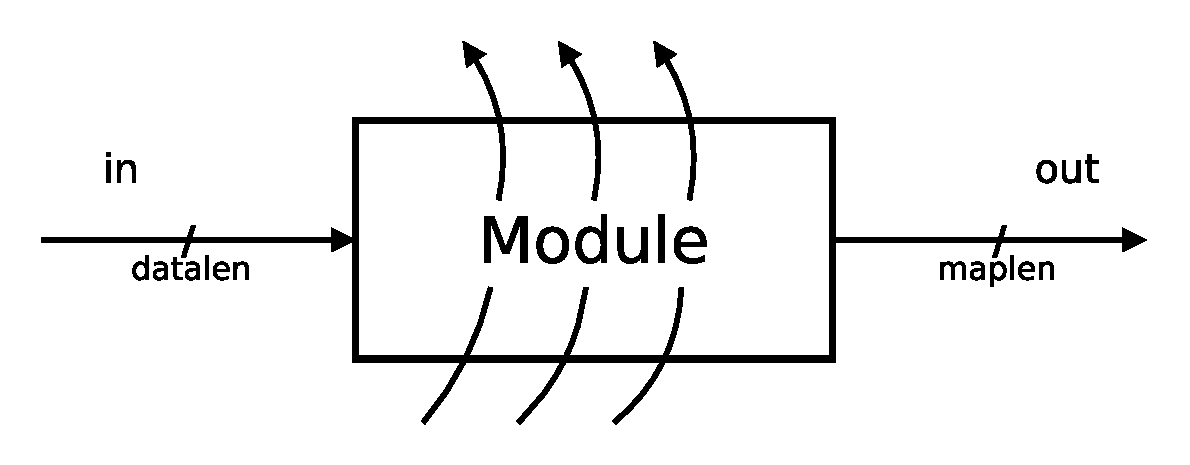
\epsfig{file=map.eps,width=0.5\columnwidth}
%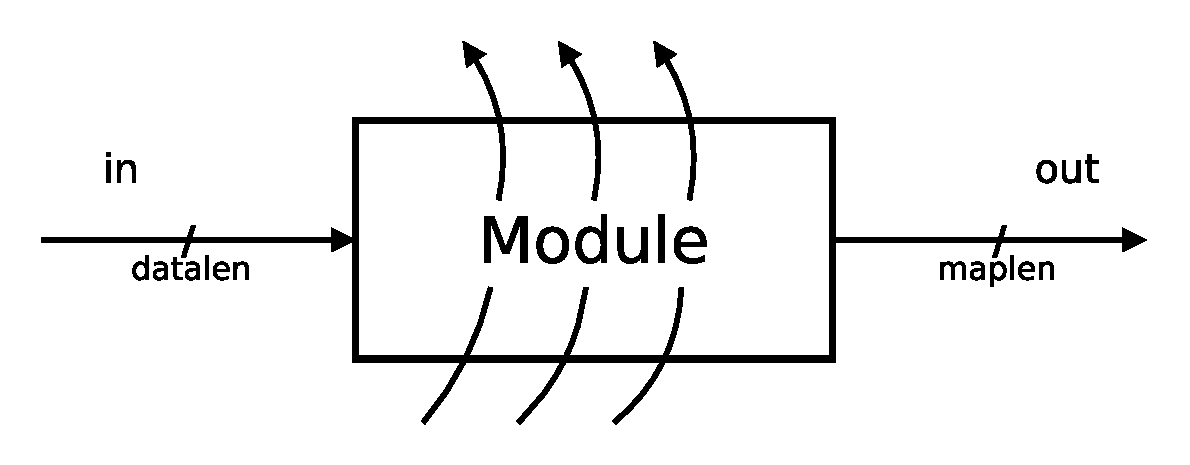
\includegraphics[scale=.5]{map}
%\vspace{-2ex}
\caption{Map Circuit Structure}
\label{fig-map}
\end{figure}
\section{Sentiment-Aspect-Region Model}
\label{sec:model}
We first present our objectives to build the
unified sentiment-aspect-region model.
To achieve the objectives, we present several intuitions
based on which we build our model.
We then describe the details of the model,
and propose a parameter estimation method.

\subsection{Intuitions}
\label{sec:motiv}
%We first introduce some notions that are used in
%explaining our objectives. There are three types of
%latent factors that are not observable in a geotagged review corpus, but
%are important for user preference analysis. They
%are topical-region, topical-aspect and sentiment.
%A topical-region represents a geographical area in which
%users do similar things (such as dining).
%%write region-specific words on their reviews.
%It comprises two components: geo-location and semantics.
%The geo-location component is usually modeled as a
%Gaussian distribution over
%POIs \cite{Yin:2011,YuanW4:2013}.
%The semantic component is modeled as a multinomial
%distribution over words \cite{Geofolk:2010}.
%Example topical-regions include shopping areas, education areas,
%streets of special snacks, etc.
%Topical-aspects are the aspects of POIs that
%are commented by users, such as environment, taste,
%price, etc. Sentiments are user's opinions over
%topical-aspects (e.g., positive, negative or neutral).
%%\KZ{Can sentiments be casted over regions? e.g., I hate
%%Clarke Quay!}
%Topical-aspects
%and sentiments can be modeled jointly \cite{JoASUM:2011}.

In this paper,
we aim at building a model that is able to 1) extract
latent variables, i.e., topical-aspect, sentiment,
and topical-region from the review
data; 2) capture the interdependencies among
category, POI, user, words and the three latent
variables; and 3) discover user's topical-region and
topical-aspect preferences.
To achieve these objectives,
we exploit the following intuitions in designing our model:

\textbf{Intuition 1}: A user visits POIs in a topical-region
because the region is geographically convenient to the user
(e.g., close to her activity areas) and its topics (e.g., shopping
street, education area, etc.) satisfy
the user's interest. Each user has her own preferences on the
topical-regions.
%We use a topical-region
%variable $r$ to model the mixture of topic and geographic
%information,
%i.e., each region exactly covers POIs of similar
%topic distribution and close in spatial.

\textbf{Intuition 2}: A user rates highly of a POI because
she likes some aspects of the POI. Such preferences might be
indicated in her review.
%i.e., user has preferences on some aspects of the POI.
Some users like to check the price range of a restaurant first while
others might be more concerned with the environment. Moreover, POIs in different
categories may have different aspects of interest.
%For
%instance, a traveler might care more about the environment
%of a hotel, while a hungry would-be diner might be more interested in
%the waiting time of a restaurant.

\textbf{Intuition 3}:
A user decides to visit a POI in a region
by considering the category, category-aware topical-aspects of the POI and
the distance to it. For example, users may visit POIs of the
restaurant category with good environment,
but she may first consider the restaurants nearby.
%to walk around a nearby shopping street.
%and visit
%POIs without being particular about the category.

\textbf{Intuition 4}: When a user writes a review on a POI, she
will use words for both the aspects of the POI and
her sentiments about the aspects.
The user may also use words for the topical-region of the POI.
For example, a review on a shop in Times Square may say:
``This shop offers best prices in Times Square.'' The reviewer
uses ``price'' for {\em aspect}, ``best'' for {\em sentiment}
and ``Times Square'' for {\em region}. %to construct the review.
%Moreover, each sentence in the review normally
%corresponds to exactly one aspect and
%users only associate one sentiment on each aspect. As a result,
%the words co-occurs in the same sentences are more likely to be correlated to
%the same aspect and sentiment.

\subsection{Model Description}
We first define the notations
to be used in the proposed model. Let $D$ be the set of user reviews,
and $U$ be the set of users. For each review, we denote the
number of its sentences by $M$ and number of words in each
sentence by $N$. In our model, a location has two attributes:
identifier and coordinates. We use $l$ to represent a location identifier
and $\boldsymbol{cd}_l$ to denote its corresponding coordinates.
Here $\boldsymbol{cd}_l$ is a latitude and longitude pair. We denote
the topical-aspect, sentiment and topical-region by $a$, $s$,
and $r$, respectively. The notations
used in this paper are listed in \tabref{tab:notation}.
Following the intuitions discussed in \secref{sec:motiv}, we
proceed to present our model.

\begin{table}[th]
\centering
%\scriptsize
\caption{Description of Symbols}
\begin{tabular}{l|l}
\hline
 Symbol & Description\\
\hline
$u$, $U$ & individual user and the set of users\\
\hline
$l$, $L$ & individual POI and the set of POIs  \\
\hline
$c$ & category  \\
\hline
$r$ & topical-region  \\
\hline
$a$, $s$ & topical-aspect and sentiment \\
\hline
$d$, $D$ & single review and the set of reviews \\
\hline
$M$ & the number of sentences in a review \\
\hline
$w$, $N$ & single word and the number of words in a sentence \\
\hline
\end{tabular}
\label{tab:notation}
\end{table}

Based on \textbf{Intuitions 1\&2}, we model the user
topical-region preferences and topical-aspect preferences
as multinomial distributions $p(r|u)$ and $p(a|u,c)$, respectively.

Based on \textbf{Intuition 3}, a user chooses a POI to visit
by considering both the category and the distance. We
define the probability of visiting a POI $l$ given
category $c$ and region $r$ proportional to $p(l|c)\cdot p(l|r)$.
Here $p(l|c)$ is the probability of selecting POI $l$ from
the category $c$; $p(l|r)$ is a the probability
of selecting POI $l$ in region $r$ by considering
the distance from $l$ to $r$. After normalization, we have the
definition $p(l|c,r)=\frac{p(l|c)p(l|r)}{\sum_{l'}{p(l'|c)p(l'|r)}}$.
%The denominator is used to normalize
%the $p(l|c)p(l|r)$ over all POIs.
To model the spatial distance, we use a
Gaussian mixture model, i.e.,
$p(l|r)\sim N(\boldsymbol{\mu}_r, \boldsymbol{\Sigma}_r)$, where
$\boldsymbol{\mu}_r$ is the center of region $r$ and
$\boldsymbol{\Sigma}_r$ is the co-variance matrix which depicts the
area of region $r$.
To model the membership of a POI to a category, we use a uniform
distribution for $p(l|c)$.
%$\kappa$ is tunable parameter used
%for balance the weights of generating POI from category and region.
%Note that $p(l|r)$ is a continuous distribution while $p(l|c)$ is
%a discrete distribution.
%To multiply the two distributions,
%we adopt the coordinate transformation approach for the Gaussian
%distribution that is proposed in Yuan et al.\cite{YuanW4:2013}.

Based on \textbf{Intuition 4},
we model the relationships among words, topical-aspects,
sentiments and topical-regions by
$p(w|a,s,r)=\lambda p(w|a,s)+(1-\lambda) p(w|r)$, where
$a$, $s$, $r$ are topical-aspect, sentiment and
topical-region, respectively.
Here $p(w|a,s)$ is the probability that the users write
word $w$ when they have sentiment $s$ on aspect $a$;
$p(w|r)$ is the probability that the users use word
$w$ to describe region $r$; parameter
$\lambda$ is used to balance the portion of
words drawn from topical-aspect, sentiment or topical-region.
We model $p(w|a,s)$ instead of $p(w|a)$ and $p(w|s)$
because aspects and sentiments are closely coupled,
and modeling by $p(w|a)$ and $p(w|s)$
needs an additional tuning parameter.
Similar to proposals of sentence level sentiment analysis
\cite{TitovMGLDA:2008,TitovMAS:2008, JoASUM:2011},
we assume each sentence expresses opinions on exactly one topical-aspect
and each topical-aspect is associated to a positive, negative or neutral sentiment.

\begin{figure}[th]
\centering
\epsfig{file=fig/modeldraft.eps,width=0.65\columnwidth}
\caption{Sentiment-Aspect-Region Model (SAR)}
\label{fig:model}
\end{figure}

In summary, the graphical representation of our model
is shown in \figref{fig:model} and
the generative process of the
reviews written by user $u$ is described as follows:
\begin{itemize}
\item For each review $d\in D_u$, where $D_u$ is the set of reviews written by user $u$.
    \begin{itemize}
    \item Draw topical region $r\sim p(r|u)$
    \item Draw category $c\sim p(c|u)$
    \item Draw location $l\sim p(l|c,r)=\frac{p(l|r)p(l|c)}{\sum_{l'}{p(l'|c)p(l'|r)}}$, where $p(l|r)\sim N(\boldsymbol{\mu}_r,\boldsymbol{\Sigma}_r)$
    \item For each sentence in review $d$
        \begin{itemize}
        \item Draw aspect $a\sim p(a|u,c)$
        \item Draw sentiment $s\sim p(s|a,l)$
        \item For each word position in the sentence
            \begin{itemize}
            \item Draw word $w\sim p(w|a,s,r)={\lambda}p(w|a,s)+(1-\lambda)p(w|r)$
            \end{itemize}
        \end{itemize}
    \end{itemize}
\end{itemize}

In the model, $p(l|c)$ and
$p(c|u)$ can be estimated directly from a given corpus. The
other distribution parameters need to be inferred.
We first present how to estimate $p(l|c)$ and
$p(c|u)$, and then show the inference algorithm for
the remaining distributions in \secref{sec:infer}.

As described in \textbf{Intuition 3},
a POI $l$ is generated from both category
and region. Since POI $l$ and category $c$ are
observable variables, we simply compute $p(l|c)$
by \equref{eq:plc}.
\begin{equation}
p(l|c)=\frac{I(l,c)}{\#\; of\; POIs\; in\; c}
\label{eq:plc}
\end{equation}
\begin{equation}
I(l,c)=
\begin{cases}
1 & l\in c \\
0 & otherwise \\
\end{cases}
\end{equation}

Similarly, we compute the category preferences of each user, i.e., $p(c|u)$,
directly from the corpus. To handle the overfitting problem,
we apply the additive smoothing technique. After smoothing, even though a user did
not a visit some category of POIs, the probability of
visiting that category still has a small value. The computation of $p(c|u)$ is shown in
\equref{eq:pcu}.
\begin{equation}
p(c|u)=\frac{n_c+\alpha}{N+{\alpha}C},
\label{eq:pcu}
\end{equation}
where $n_c$ is the number of reviews of POIs in category $c$ that user $u$
writes; $N$ is the total number of reviews on POIs in $c$; $C$
is the total number of categories; $\alpha$  is the smoothing
parameter which is usually set to a value smaller than 1. In this paper,
we set $\alpha=0.1$.

\subsection{Inference Algorithm}
\label{sec:infer}
To infer the parameters of the model, we
use the expectation-maximization (EM) approach.
In this section,
we present the computation of the corpus
likelihood, the two-step EM algorithm
used to infer our parameters, and
initialization of the EM algorithm.

\subsubsection{Likelihood Computation}
Our model has several levels, i.e., word level,
sentence level, and document level. The latent variables
are on two levels. Region $r$ is at document level while
aspect $a$ and sentiment $s$ are at sentence level.
This multi-level structure poses challenges to the estimation of
the log-likelihood. According to the generative
process, we have the likelihood of the corpus $D$:
\begin{equation}
p(D;\Phi)=\prod_{d}^{D}{p(u_d)\sum_{r}^{R}{p(r|u_d)}p(l_d,\mathbf{w}_d|r,u_d)}
\label{eq:likeli1}
\end{equation}
\begin{equation}
p(l_d,\mathbf{w}_d|r,u_d)=p(c_{l_d}|u_d)p(l_d|r,c_{l_d})\prod_{i}^{M}{p(\mathbf{w}_{d,i}|c_{l_d},r,u_d,l_d)}
\label{eq:likeli2}
\end{equation}
\begin{equation}
\begin{split}
&p(\mathbf{w}_{d,i}|c_{l_d},r,u_d,l_d) \\
&=\sum_{a,s}{p(a|c_{l_d},u_d)p(s|a,l_d)\prod_{j}^{N}{p(w_{d,i,j}|a,s,r)}}
\end{split}
\label{eq:likeli3}
\end{equation}
In \equref{eq:likeli1}, $\Phi$ is the set of parameters in the model,
i.e., $p(r|u)$, $p(a|c,u)$,$p(l|r)$,$p(s|a,l)$,$p(w|a,s)$,
$p(w|r)$,$\boldsymbol{\mu}_r$ and $\boldsymbol{\Sigma}_r$.
Variables $u_d$,$l_d$,$\mathbf{w}_d$ are the user, location and
words of review $d$, respectively. Variable $\mathbf{w}_{d,i}$
represents the set of words in sentence $i$ of review $d$
while $w_{d,i,j}$ is the $j^{th}$ word in sentence
$i$ of review $d$. Taking logarithm of
$p(D;\Phi)$ leads to a summation inside the logarithm:
\begin{equation}
L=\sum_{d}{\log{p(u_d)}+\log{\sum_{r}{p(r|u_d)p(l_d,\mathbf{w}_d|r,u_d)}}}
\label{eq:loglikeli}
\end{equation}
Since this likelihood cannot be estimated directly,
we adopt Jessen's
inequality to the log-likelihood, and estimate the
lower bound of the likelihood and the parameters
in an iterative manner.

\subsubsection{Expectation-Maximization}
Due to the aforementioned difficulty of computing
log-likelihood directly,
we apply Expectation-Maximization (EM)
algorithm to estimate the model parameters.

In \textbf{E-step}, we compute the expectation
of latent variables given the observed data.
By applying Jessen's inequality to \equref{eq:loglikeli},
we get the lower bound of the likelihood as:
\begin{equation}
\begin{split}
L_{LB}=&\sum_{d}{\log{p(u_d)}}\\
+&\sum_{d,r}{p(r|d)(\log{p(r|u_d)}+\log{p(l_d,\mathbf{w}_d|r,u_d)})}
\end{split}
\label{eq:loglikeli1}
\end{equation}
As shown in \equref{eq:loglikeli1},
we need to estimate $p(r|d)$ to compute the full likelihood.
We apply Bayes rule, and obtain the update
function of the posterior distribution as
\begin{equation}
p(r|d)=\frac{p(r,d)}{\sum_{r}{p(r,d)}}
\label{eq:prd}
\end{equation}
\begin{equation}
p(r,d)=p(u_d)p(r|u_d)p(l_d,\mathbf{w}_d|r,u_d)
\label{eq:prdjoint}
\end{equation}
In \equref{eq:prdjoint},
$p(l_d,\mathbf{w}_d|r,u_d)$ is computed by \equref{eq:likeli2}, and
$p(u_d)$ appears both in the numerator and the denominator,
and thus is not necessary to estimate.

In \textbf{M-step}, by maximizing the lower bound of likelihood,
we can obtain the update function of parameters at document level
that are related to topical region $r$ as below.
\begin{equation}
p(r|u)=\frac{\sum_{d\in D_u}{p(r|d)}}{\sum_{r}{\sum_{d\in D_u}{p(r|d)}}}
\label{eq:pru}
\end{equation}
%\begin{equation}
%\boldsymbol{\mu}_r=\frac{\sum_{d}{p(r|d)\cdot \boldsymbol{cd}_{l_d}}}{\sum_{d}{p(r|d)}}
%\label{eq:mu}
%\end{equation}
%\begin{equation}
%\boldsymbol{\Sigma}_r=\frac{\sum_{d}{p(r|d)\cdot (\boldsymbol{cd}_{l_d}-\boldsymbol{\mu}_r)^T(\boldsymbol{cd}_{l_d}-\boldsymbol{\mu}_r)}}{\sum_{d}{p(r|d)}}
%\label{eq:sigma}
%\end{equation}

However, we cannot obtain a close form solution for $\boldsymbol{\mu}_r$ and
$\boldsymbol{\Sigma}_r$ due to the normalization term. We adopt a gradient method
to obtain the update value of $\boldsymbol{\mu}_r$ and $\boldsymbol{\Sigma}_r$ in M-step.
Specifically, we use the BFGS quasi-Newton method \cite{Kurashima:2013,Liu:1989}.
In the gradient method, we compute the gradient of $\boldsymbol{\mu}_r$ and
$\boldsymbol{\Sigma}_r$ as follows:
\begin{equation}
\frac{\partial L_{LB}}{\partial \boldsymbol{\mu}_r}=
\sum_d{p(r|d)\boldsymbol{\Sigma}_r^{-1}\left(\frac{\sum_{l'}{q(l')(\boldsymbol{cd}_{l'}-\boldsymbol{\mu}_r)}}{\sum_{l'}{q(l')}}-
(\boldsymbol{cd}_{l_d}-\boldsymbol{\mu}_r)\right)}
\label{eq:gmu}
\end{equation}
\begin{equation}
\frac{\partial L_{LB}}{\partial \boldsymbol{\Sigma}_r}=\sum_d{p(r|d)(\frac{\sum_{l'}{q(l')g(l', r)}}{\sum_{l'}{q(l')}}-g(l_d, r))}
\label{eq:gsigma},
\end{equation}
%\begin{equation}
%g(l, r)=-\frac{1}{2}\boldsymbol{\Sigma}_r^{-1}+\frac{1}{2}\boldsymbol{\Sigma}_r^{-1}(\boldsymbol{cd}_{l}-\mu_r)(\boldsymbol{cd}_{l}-\mu_r)^T\boldsymbol{\Sigma}_r^{-1}
%\end{equation}
where $q(l')=p(l'|c_l)p(l'|r)$ and $\boldsymbol{cd}_{l}$ denotes the coordinates of POI $l$.
The function $g(l, r)$ in \equref{eq:gsigma} is the gradient of the Gaussian distribution for region $r$
w.r.t. $\boldsymbol{\Sigma}_r$ at point $l$.

Since sentiment and aspect are at the sentence level, we
cannot compute $\log p(l_d,\mathbf{w}_d|r,u_d)$
in \equref{eq:loglikeli1} using $p(r|d)$. 
Thus, we propose a second level of EM iterations.
Specifically, we introduce a new latent variable to estimate parameters related to
aspect and sentiment. Specifically, we use $\phi_{a,s,r,d_i}$ to identify
the probability that the $i^{th}$ sentence in a review $d$ from
region $r$ is assigned with aspect $a$ and sentiment $s$.
we use $\phi_{a,s,r,d_i}$ and $p(r|d)$ to compute the update
function of $p(a|c,u)$, $p(s|l,a)$,
$p(w|a,s)$, and $p(w|r)$.

Denote by $n(w,d_i)$ the number of occurrences of word $w$ in sentence $i$
of review $d$. We estimate $\phi_{a,s,r,d_i}$ as:
\begin{equation}
\phi_{a,s,r,d_i}=\frac{p(a,s,r,d_i)}{\sum_{a,s}{p(a,s,r,d_i)}}
\label{eq:pasrdi}
\end{equation}
\begin{equation}
\begin{split}
p(a,s,r,d_i)=p(u_d)p(r|u_d)p(c_{l_d}|u_d,r)p(l_d|r,c_{l_d})\\
p(a|c_{l_d},u_d)p(s|a,l_d)\prod_{w}{p(w|a,s,r)^{n(w,d_i)}}
\end{split}
\end{equation}

By maximizing the lower bound of the likelihood, we
obtain the update function of the rest parameters:
\begin{equation}
p(a|u,c)=\frac{\sum_{d\in D_u}{\sum_{r}{p(r|d)\sum_{i}{\sum_{s}{\phi_{a,s,r,d_i}}}}}}{\sum_{a'}{\sum_{d\in D_u}{\sum_{r}{p(r|d)\sum_{i}{\sum_{s}{\phi_{a',s,r,d_i}}}}}}}
\label{eq:pacu}
\end{equation}
\begin{equation}
p(s|l,a)=\frac{\sum_{d\in D_l}{\sum_{r}{p(r|d)\sum_{i}{\sum_{s}{\phi_{a,s,r,d_i}}}}}}{\sum_{s'}{\sum_{d\in D_l}{\sum_{r}{p(r|d)\sum_{i}{\sum_{s}{\phi_{a,s',r,d_i}}}}}}}
\label{eq:psal}
\end{equation}
\begin{equation}
p(w|s,a)=\frac{\sum_{d}{\sum_{r}{p(r|d)\sum_{i}{\phi_{a,s,r,d_i}n(w,d_i)}}}}{\sum_{w'}{\sum_{d}{\sum_{r}{p(r|d)\sum_{i}{\phi_{a,s,r,d_i}n(w',d_i)}}}}}
\label{eq:pwsa}
\end{equation}
\begin{equation}
p(w|r)=\frac{\sum_{d}{p(r|d)\sum_{i}{\sum_{a}{\sum_{s}{\phi_{a,s,r,d_i}n(w,d_i)}}}}}{\sum_{w'}{\sum_{d}{p(r|d)\sum_{i}{\sum_{a}{\sum_{s}{\phi_{a,s,r,d_i}n(w',d_i)}}}}}},
\label{eq:pwr}
\end{equation}
where $D_u$ is the set of reviews written by user $u$ and $D_l$
is the set of reviews for POI $l$.

\subsubsection{Initialization of EM Algorithm}
EM algorithm can only guarantee to find a local optima.
Different initializations may lead to different results.
In this section, we present our methods for initializing the assignment of
aspect, sentiment and region.

\textbf{Aspect} is extracted from sentence level in our model.
We initialize the aspect by a clustering process on
sentences. Each sentence is represented as a vector of words.
Given the number of aspects, we use K-means clustering
algorithm to assign each sentence an aspect.
We then initialize $p(w|a)$ by the probability that word
$w$ appears in sentences carrying aspect $a$.

\textbf{Sentiment} has 3 possible values in this paper:
positive, negative and neutral.
In order to know the polarity of each sentiment, we need some prior
knowledge. We use the same predefined set of sentiment seed words
as in Jo's proposal \cite{JoASUM:2011}. Moreover, we apply a syntactic parser to
extract negation of the sentiment words such as ``not good'' and
use a special word ``not\_good'' to represent the phrase ``not good''
in our vocabulary. For each word in the seed word set, we assign
a probability ($p(w|s)$) of 1 to its polarity and 0 to the other
two polarities. For words not in the seed word set, we assign an
equal probability for each polarity. We then use $p(w|a)p(w|s)$
to approximate $p(w|a,s)$.

\textbf{Region} is initialized by a K-means clustering
algorithm based on the coordinates (latitude and longitude).
The clustering algorithm partitions POIs to different
regions. Then for each region r, we compute $\boldsymbol{\mu}_r$
and $\boldsymbol{\Sigma}_r$ using a regression
over the POIs in the region.
We compute $p(w|r)$ by the distribution of
words in the reviews for POIs in region $r$ and $p(r|u)$ by the
portion of reviews that user $u$ writes in region $r$.

For other parameters: $p(a|c,u)$ and $p(s|a,l)$, we initialize
them by using the assignment of aspect and sentiment to a sentence
(We assign sentiment to a sentence by voting from sentiment seed words
extracted from the sentence). Specifically, $p(a|c,u)$ is proportional to the
number of sentences that are assigned to $a$ and that belong to a review
written by $u$ from category $c$; $p(s|a,l)$ is proportional to
the number of sentences that belong to location $l$ and
are assigned to sentiment $s$ and aspect $a$ at the same time.

\subsubsection{Efficiency Analysis}
Let the number of sentiment be 3 and we treat it as
constant. In E-step,
the computation of the expectation of latent variables in \equref{eq:prd}
and the variables $\phi_{a,s,r,d_i}$ in \equref{eq:pwr}
needs $O(|D|MNRA)=O(WRA)$, where $W$ is the number of words in the reviews of all
users' in training set,
$R$ is the number of regions and $A$ is the number of aspects.
In M-step, the cost for updating \equref{eq:pacu} to (\ref{eq:pwr})
is $O(UA+LA+VA+VR)$,
where $U,L,V$ are the number of users, POIs and unique words, respectively.
To update $\boldsymbol{\mu}$ and $\boldsymbol{\Sigma}$, we perform a
quasi-Newton method. Since each $\boldsymbol{\mu}_r$ and $\boldsymbol{\Sigma}_r$
are two dimensional vector and $2\times2$ matrix, respectively. The computation cost of matrix operation
can be treated as constant. Let $D$ be the number of reviews, the cost of
computing gradient in \equref{eq:gmu} and (\ref{eq:gsigma})
is $D+L$.
Therefore, the complexity of quasi-Newton is $O(I_qR(D+L))$, where $I_q$
is the number of iterations of quasi-Newton.
In summary, the total complexity of the learning
algorithm with $I$ iterations is $O(I(WRA+I_qR(D+L)+UA+LA+VA+VR))$.
Since $WRA\gg (UA+LA+VA+VR)$, we simplify the cost as $O(I(WRA+I_qR(D+L)))$.
%The training complexity is high, but
%fortunately, the training process can be done offline,
We can parallelize the computation
of both E-step and M-step. In E-step, since
the computation of $p(r|d)$ on each document is independent to others, we can compute $p(r|d)$
of each document in parallel. In M-step, the update of \equref{eq:pacu} to (\ref{eq:pwr}) and
the quasi-Newton iterations can also be
parallelized in the similar way as $p(r|d)$. Therefore, the algorithm can be fully parallelized.

\section{Applications}
\label{sec:app}
%Our model can be applied to POI recommendation and user recommendation.
%We show in detail how to use the estimated parameters for recommendation.
We present three applications of our model, namely POI recommendation,
user recommendation, and aspect satisfaction analysis in regions. In POI recommendation,
we provide a way to explain the reason of recommending a POI and
propose an efficient online recommendation algorithm.
% region-aware users' satisfaction estimations.

\subsection{POI recommendation}
\label{sec:model-poirec}
%Most of the existing proposals for POI recommendation are
%based on collaborative filtering.
%Ye et al. \cite{YeGeoSocial:2011} propose a fusion framework to
%combine user-based, friend-based and geo-based collaborative
%filtering. In the geographic model, the probability of transporting
%from one POI to another is drawn from a power law distribution over
%the distances between the two POIs. The probability of a user
%visiting a POI is given by considering the distances between the
%POI and the POIs visited by the user. Yuan et al.
%\cite{YuanPOI:2013} propose a time-aware model
%for recommendation where check-ins
%are divided into different groups by different time segments to
%model user interests by time. Yang et al. \cite{YangSenti:2013}
%propose a sentiment-enhanced location recommendation
%system. They combine both check-ins and
%the overall sentiment on each location
%and apply probabilistic matrix factorization for recommendation.
%Different from these proposals, our model recommends POIs based
%on user topical-aspect preferences, topical-region preferences
%and the aspect-level sentiment of the POIs.

We apply our model to two POI recommendation tasks
and propose an efficient online recommendation algorithm.
The two recommendation tasks are \emph{All-Category Recommendation}
and \emph{Single-Category Recommendation}.

\subsubsection{All-Category Recommendation}
All-Category Recommendation is a task of
generating a rank list of POIs in any category
given a set of POIs and a user.
%When
%a user wants to visit a place without specifying the category,
%she needs recommendation from all of the categories.
The aforementioned proposals are all for all-category recommendation.
We calculate the
probability of $p(l,s_+|u)$, i.e., the probability of user
$u$ visits POI $l$ with positive sentiment, to score $l$ for $u$
as shown in \equref{eq:poiacr}.
\begin{equation}
\begin{split}
p(l,s_+|u)=&\sum_{r}{p(r|u)p(c_l|u)p(l|r,c_l)}\\
&\sum_{a}{p(a|u,c_l)p(s_+|a,l)}
\label{eq:poiacr}
\end{split}
\end{equation}
According to \equref{eq:poiacr}, we make the recommendation
by considering the matching between user preferences (i.e., $p(r|u)$,
$p(c_l|u)$ and $p(a|u,c_l)$) and the attributes of the POI
(i.e., $p(s_+|a,l)$ and $p(l|r,c_l)$).
%Only when the location satisfy the preference, i.e., the probabilities
%$p(s_+|a,l)$ and $p(l|r)$ are high for the user's preferred aspects $a$
%and region $r$, will $l$ be probably visited
%and satisfied by user $u$.
%In summary, our model considers aspect($p(a|u,c)$),
%sentiment($p(s_+|a,l)$) and region($p(r|u)p(l|r)$) when
%giving a recommendation.

This recommendation model enables us to explain why we recommend
a POI to a user. We consider two factors: aspect and region.
First, we rank the aspects by $p(s_+|a,l)p(a|u,c_l)$ to reveal
which aspects match the user's preferences.
Second, we rank the regions by $p(r|u)p(l|r)$ to reveal which regions
contribute more to the recommendation. Finally, we choose top several
aspects and regions for explanation.

\subsubsection{Single-Category Recommendation}
Single-Category Recommendation aims at
ranking POIs given a user and
a specific category (e.g., restaurants).
It is a typical scenario for POI recommendation
although it has not been covered in previous work.
We compute $p(l,s_+|u,c)$ as shown in \equref{eq:poiscr}.
Compared to all-category recommendation, we fix the category
i.e., remove $p(c|u)$ from \equref{eq:poiacr}.
All locations that are not in $c$ will not be
considered in this scenario.
\begin{equation}
\begin{split}
p(l,s_+|u,c)=&\sum_{r}{p(r|u)p(l|r,c)}\\
&\sum_{a}{p(a|u,c)p(s_+|a,l)}
\label{eq:poiscr}
\end{split}
\end{equation}
We can also offer explanation for the single-category recommendation
by following similar method as we employ for the all-category recommendation.

\subsubsection{Efficient algorithm for Top-N Online Recommendation}
Time efficiency is an essential part of online recommendation. A straightforward
method of making recommendation is to compute the recommendation score as \equref{eq:poiacr}
or \equref{eq:poiscr}.
This method requires traversing all the regions which is highly time consuming.
Another choice is the threshold algorithm \cite{FaginTA:2001}
that may save the computation for some POIs.
However, in our applications, the
number of attributes (i.e., regions and aspects) is large, and thus it is expensive
to compute the recommendation score even for a single POI.
The threshold algorithm cannot help with this, either.
We propose an optimized top-N items recommendation algorithm that significantly
reduces the time cost. As to be shown in the experiment,
our algorithm is faster than the threshold algorithm
in the top-N POI recommendation using our model. Our algorithm
can be applied to all or single-category POI recommendation. % as well as user recommendation.
We use all-category POI recommendation (\equref{eq:poiacr})
as an example to explain the algorithm.

Our algorithm is based on two observations:
1) A user only prefers a small number of regions;
and 2) POIs in the center of the
region are more likely to be recommended. These two observations indicate that only when
a user prefers a region and the POI is near the center of the region, will the score
$p(r|u)p(l|r,c_l)$
contribute significantly to the recommendation score.
Therefore, after we have computed the most possible regions for a POI,
it may not be necessary to compute the remaining regions.
We design a branch and bound algorithm as shown in Algorithm \ref{oprec}
to prune the search space of the regions.
Our algorithm contains two steps: \emph{initialization} and \emph{pruning}.
%By using the second observation, we can produce a
%good initial top-N list.

%Consider the POI recommendation mentioned in \equref{eq:poiacr}.
In the \emph{initialization} step (line 2),
we find $N$ candidate POIs that are potentially
good for recommendation.
Specifically, we pick top $K$ regions which
cover most of the user's regional preferences
(i.e., $\sum_{i=1}^{K}{p(r_i|u)}>0.9$) with smallest $K$ (line 21).
If $K$ is larger than $N$, we pick at most $N$ regions
to ensure that we can select at least one candidate from each region.
In each of the top $K$ region, we choose top $\ceil*{\frac{N}{K}}$
POIs w.r.t. $p(l|r)$ as candidates.

In the \emph{pruning} step (line 9-10),
we check whether we can avoid traversing unnecessary regions for each POI.
%we check whether there is a POI that
%has a larger recommendation score than the smallest one in the candidate set.
%To compute the recommendation score, we need to traverse all regions
%to sum up $p(r|u)p(l|r,c_l)$ for each POI in the straightforward method.
We traverse the regions according to
the descending order of $p(l|r,c_l)$ for POI $l$. Suppose we have traversed regions
$\{r_1,...,r_{i-1}\}$. The partial score we have computed for the traversed regions is
\[PScore=\sum_{j=1}^{i-1}{p(r_j|u)p(l|r_j,c_l)}.\]
When we explore the i-th region, we compute the upper bound of
recommendation score for the POI as:
\begin{equation}
\label{eq:bound}
Bound^{(i)}(l)=PScore+(1-\sum_{j=1}^{i-1}{p(r_j|u)})p(l|r_i,c_l).
\end{equation}
%and $\sum_a{p(s_+|a,l)p(a|u,c_l)}=1$

Because we check the regions in the descending
order of $p(l|r,c_l)$, the actual value of $p(l|r,c_l)$
for the remaining regions should be less than the one
for the current region, i.e., $p(l|r_i,c_l)$.
Therefore, we have a partial recommendation
score for the rest of the regions, which is at most
\[(1-\sum_{j=1}^{i-1}{p(r_j|u)})p(l|r_i,c_l),\]
where
$1-\sum_{j=1}^{i-1}{{p(r_j|u)}}$ is the portion of user preferences for
the rest regions. The upper bound of
$\sum_r{p(l|r,c)p(r|u)}$ for all regions is
$PScore+(1-\sum_{r=r_1}^{r_{i-1}}{p(r|u)})p(l|r_i,c_l)$.
Since $\sum_a{p(a|u,c)p(s_+|a,l)}\le1$,
Finally, we obtain the upper bound of the recommendation score in \equref{eq:poiacr}
for the POI
by setting $\sum_a{p(a|u,c)p(s_+|a,l)}=1$, which results in
\equref{eq:bound}.

If the upper bound
is smaller than the $N^{th}$ candidate (Line 9),
we skip the current POI (no need to check the remaining regions).
Otherwise, we continue to check the
remaining regions.
If all regions are examined for the POI and the POI is not pruned by the aforementioned
upper bound, we compute the full score
of the POI to compare with the $N^{th}$ smallest candidate (line 12).
We remove the $N^{th}$ candidate
in the list and insert the POI to the list if the full score is
larger than the $N^{th}$ candidate (line 13-15). To maintain the
top-N candidate list, we use a binary min-heap.
%Details are shown in Algorithm \ref{oprec}.

\begin{algorithm}[th]
\caption{POI Recommendation}
\label{oprec}
\begin{algorithmic}[1]
\Function{Rec}{u, N}
\State {$H \leftarrow InitialCandidates(N)$}
\For {$l\in L\;and\;l\not\in H$}
\State $PartS \leftarrow 0, PartRPro\leftarrow 0, Skip\leftarrow false$
\While {there exists $r$ not examined for $l$}
\State {$r\leftarrow NextRegion()$}
\State {$PartS\leftarrow PartS+ p(r|u)p(l|r,c_l)$}
\State {$PartRPro\leftarrow PartRPro+ p(r|u)$}
\If {$PartS+(1-PartRPro)*p(l|r,c_l)<H.Top()$}
\State $Skip\leftarrow true, break$
\EndIf
\EndWhile
\If {$Skip=false$}
\State {$S\leftarrow PartS * p(c_l|u)\sum_a{p(s_+|a,l)p(a|u,c_l)}$}
\If {$S>H.Top()$}
\State {$H.DeleteTop()$}
\State {$H.Insert(<l,S>)$}
\EndIf
\EndIf
\EndFor
\State $Result\leftarrow\; Sort\; H\; by\; Score\; S$
\State \textbf{return} $Result$
\EndFunction
\Statex
\Function{InitialCandidates}{N}
\State {$H\leftarrow \emptyset$}
\State $r_1,...,r_R\leftarrow$ Sort the regions by $p(r|u)$
\State Pick top $K$ regions satisfies: $K=min(\{k|\sum_{i=1}^{k}{p(r_i|u)}>0.9\},N)$ %1) $\sum_{i=1}^K{p(r_i|u)}>0.9$; or 2) $K=N$
\State From $r_1$ to $R_K$, Insert top $\ceil*{\frac{N}{K}}$ POIs ordered by $p(l|r)$ to $H$ until $H$ contains $N$ POIs
\State \textbf{return} $H$
\EndFunction
\end{algorithmic}
\end{algorithm}

\subsection{User Recommendation}
We can also apply our model to recommend
users for a POI. Predicting which users may favor a given
POI is useful when the owner of the POI wants to target at or advertise
to some of the users.
%The users who favor the POI probably
%write positive reviews to the POI, which may then increase the
%overall ratings and attracts more users. User recommendation
%can be treated as an inverse process of POI recommendation.
%The goal is to generate a user list for
Given a POI $l$, we
compute the probability $p(u,s_+|l)$
of user $u$ favoring POI $l$ by considering both topical-region
and topical-aspect preferences of users as follows:
\begin{equation}
p(u,s_+|l)=\frac{p(u,s_+,l)}{\sum_{u,s}{p(u,s,l)}}
\label{eq:puspl}
\end{equation}
\begin{equation}
\begin{split}
p(u,s,l)=&p(u)p(c_l|u)\sum_{r}{p(r|u)p(l|r,c_l)}\\
&\sum_{a}{p(a|u,c_l)p(s|a,l)},
\end{split}
\label{eq:pusl}
\end{equation}
%Similar to POI recommendation, we also consider user's
%topic and aspect preferences. In additional to the two
%preferences, the computation in \equref{eq:pusl}
%involves $p(u)$ which
%is exactly proportional to contribution of user $u$.
%A user who is active to write reviews are more likely to
%write reviews to POI that she visits next. This user
%should be recommended to the POI with higher probability
%than inactive users.
where prior $p(u)$ is calculated
using the user's review history:
\[p(u)=\frac{\#\; of\; reviews\; u\; wrote}{\#\; of\; all\; reviews}.\]
Since the last two summations are the same as those in
POI recommendation,
Algorithm \ref{oprec} can also be used to speed up the user recommendation.

\subsection{Aspect Satisfaction Analysis in Regions}
\label{sec:asr}
Discovering which aspect is satisfied or not by
users in each region is useful when 1) someone wants to
set up a new business or make strategies to attract more customers,
or 2) policy makers make urban planning.
For example, most of the restaurants in a region
of a city may be complained for the
long waiting time. By knowing the dissatisfaction of this aspect,
a restaurant may think how to achieve competitive
advantage over other restaurants in the region.
We can infer the aspect satisfaction
in each region based on our model. Specifically, we compute the
aspect distribution of each sentiment $s$, category $c$ and
region $r$ as
\begin{equation}
%p(s|a,c,r)=\sum_{l}{p(s|a,l)p(l|r)p(l|c)}
p(a|s,c,r)=\frac{\sum_{u,l}{p(u)p(r|u)p(c|u)p(a|c,u)p(l|r,c)p(s|a,l)}}{
\sum_{a,u,l}{p(u)p(r|u)p(c|u)p(a|c,u)p(l|r,c)p(s|a,l)}}
\label{eq:sat}
\end{equation}
This probability shows which aspect is most probably liked/disliked
in POIs from category $c$ and region $r$.
%The weighted-sum of user
%aspect preferences $p(a|c,u)$
%in \equref{eq:sat} give higher weight for aspect that often mentioned
%by users who are active in the region.


%\section{Variational Message Passing}

Let $\Theta$ be the set of hidden variables and $X$ be the observed variables.
parametric family of distributions. We use capital letters $P$, $Q$ to
represent distributions, and corresponding small letters $p$, $q$ to denote
its probabilistic density function or probability mass function.
Variational inference approximates the posterior distribution
$P_{\Theta|X}$ with a distrbution $Q_{\Theta}$ from a
A simple choice of the
approximating
family is,
\begin{equation*}
	q(\Theta) = \prod_{\theta \in \Theta} q(\theta)
\end{equation*}
, the fully factorized family over the parameters. This choice assumes that
all hidden variables are independent in the approximate distribution. Since
the independence assumption may not be true in the posterior distribution, the
algorithm may not be able to find the exact posterior distribution. The
algorithm iteratively minimizes the Kullback-Leibler divergence
$\mathrm{KL}(Q||P)$ between the approximate distribution and
the true distribution so that the approximate distribution is as close as
possible to the true posterior. Although the KL divergence cannot be computed
without knowing the true posterior, it is not necessary to
directly optimize the KL divergence. Instead, the algorithm maxmizes the
evidence lower bound (ELBO) 
\begin{equation}
	\label{eqn:ELBO}
	\mathcal{L}(Q) = E_Q[\ln p(\Theta, X) - \ln q(\Theta)] 
\end{equation} 
, maximizing which is equivalent to minimizing the KL divergence. ELBO only
involves the expectation of the log likelihoods in terms of the approximate
distribution $Q$ and it is straight forward to calculate. 

Separating out terms related to one of the hidden variables $\theta \in
\Theta$ and let $F_{(\cdot)}$ be the parent of the variable and
$\mathrm{C}_{(\cdot)}$ be the set of children of the variable, the ELBO can be
rewritten as
\begin{align*}
	&\mathcal{L}(Q) = -\mathrm{KL}(Q_\theta || \tilde{P}_\theta) +
	\mathrm{Const}(\theta) \numberthis \label{eqn:ELBO_one_term}
\end{align*}
, where $\mathrm{Const}(\theta)$ is a constant with respect to $\theta$ and $\tilde{P_\theta}$ is defined as
\begin{align*}
	&\ln\tilde{p}(\theta) = E_{Q_{\Theta \backslash
	\theta}}[\ln p(\theta|\mathrm{F}_\theta) + \sum_{\phi \in
	\mathrm{C}_\theta }p(\phi|\mathrm{F}_\phi)] + Z
\end{align*}
$Z$ is a normalizing constant. The KL divergence is always non-negative. It
equals to zero if and only if the two distributions are the same. Therefore,
setting $Q_\theta$ to $\tilde{P}_\theta$ maximizes the ELBO with regard to
$\theta$.  Since the model is in exponential family and have conjugate priors,
all terms in $\ln \tilde{p}(\theta)$ has the same form of the dot product of
parameters and sufficient statistics except the normalizing constant.
Therefore, the ELBO is maximized by letting $\ln q(\theta)$ have the same form
as $p(\theta|\mathrm{F}_\theta)$ and setting the parameters to those of
$\tilde{P_\theta}$.  In the coin flipping case, if the probability of head has
$\mathrm{Beta}(\alpha, \beta)$ prior,
\begin{align*}
\ln\tilde{p}(\phi) &= [\alpha - 1 \quad \beta - 1] 
	\begin{bmatrix} \ln \phi \\ \ln(1-\phi) \end{bmatrix}  \\
	&+ [H \quad N-H]  \begin{bmatrix} \ln \phi \\ \ln(1-\phi) \end{bmatrix} + Z
\end{align*}
The ELBO is maximized when the $Q$ is set to $\mathrm{Beta}(\alpha + H,
\beta + N - H)$. Note in the one coin model, $Q$ is exactly the true
posterior in \eqnref{eqn:coin_posterior} because the independence assumption
naturally holds for a univariate distribution.

\begin{figure}[h]
	\includegraphics[scale=0.5]{figs/two_coins_latent.eps}
	\label{fig:two_coins_latent}
	\caption{Introducing additional hidden variables to mixture model}
\end{figure}

Mixture models (e.g. flipping two coins) are no longer in Exponential conjugate
family. To apply the variational algorithm, the trick is to introduce
additional hidden variables. For example, we can add the choice of the coins
(i.e. $z_i$ in \figref{fig:two_coins_latent}) for each of the outcomes. Let
$z_{ik} = 1$ if $z_i = k$, $z_{ik} = 0$ otherwise, and $x_{i} = 1$ if $x_i$ is
head, $x_{i} = 0$ if $x_i$ is tail, the log likelihood of
$x_i$ is 
\begin{align*}
	\ln p(x_i|\phi_1, \phi_2, z_i) = \sum_{k=1}^2 z_{ik} [x_{i} \quad 1-x_{i}]
\begin{bmatrix} \ln \phi_k \\ \ln (1-\phi_k) \end{bmatrix}
\end{align*}
The log likehood has the same forms as the prior $\ln f(\phi_k; \alpha, \beta)$.
Hence the model is conjugate.

The updates to the parameters of approximate distributions $Q$
are the aggregation of terms that either only depends on the parent or depends
on one child and the other parents of it. The terms in the updates can be
computed locally at the neighbours of the updated random variable.  For
example, the update of $z_i$'s parameters in the
two coins model is
\begin{equation}
	E[\ln \pi] + E[\ln p(x|\phi)]
\end{equation}
The first term can be computed locally at $\pi$ and the second term can be
computed locally at $x_i$ given $\phi_1$ and $\phi_2$.  The VMP algorithm
defines the terms as messages to be sent along both directions of edges in the
Bayesian network. In each step, one of the vertecies is chosen to pull
messages from its neighbours and update itself by aggregating the messages.
If a message is from the child and also depends on co-parents, the child will
pull messages from the co-parent as well. 

%\section{Circuit Component and Generator}\label{sec:syntax}
We explored the reconfigurable circuit component in AES architecture and designed a
new language construct $map$ accordingly to describe it, which portraits the computation 
meaning of the reconfigurable structure.

The $map$ is used to model the circuit that does some operations upon a list of data. It's also similar to higher order function "$map$" in Haskell. In Haskell, $map$ takes two inputs - a function, and a list. It then applies this function to every element in the list. In Verilog we don't have list type. However we can view a $reg$ or $wire$ as a bit list, and every time we applies the function (actually we should call it a $module$ in circuit design) to a slice of the bits. Figure \ref{fig-map} shows the $map$ structure, as an example, we can think  "Module" has the functionality that adds 1 to the input data list. Here comes the syntax of $map$:

\begin{verbatim}
         map(md,data,datalen,maplen)
\end{verbatim}
where $md$ is a module identifier, $data$ is the bit-list name (variable name of a $reg$ or $wire$), $datalen$ is the length of the bit-list and $maplen$ is the length of the bit slice that applied to the module each time.
%\vspace{-2ex}
\begin{figure}[ht]
\centering
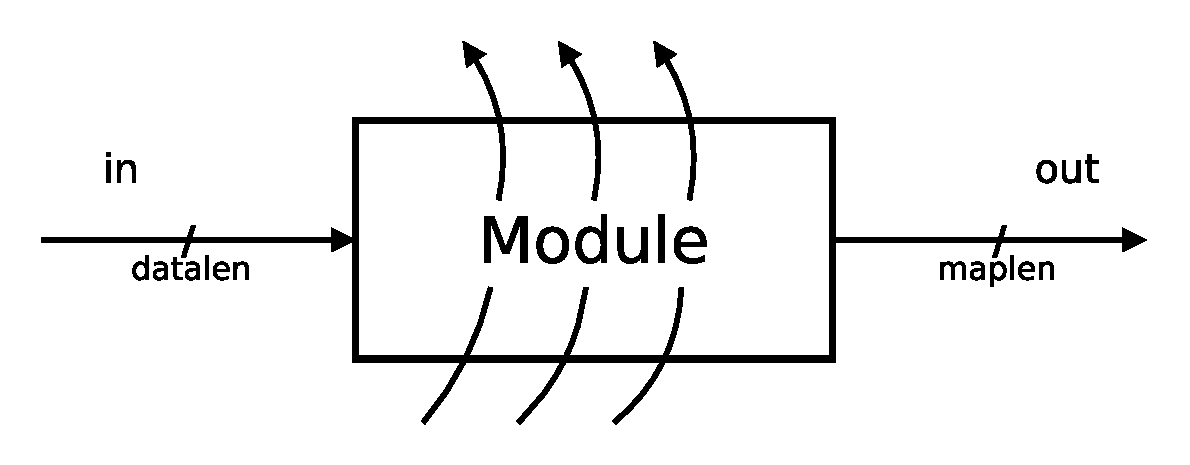
\epsfig{file=map.eps,width=0.5\columnwidth}
%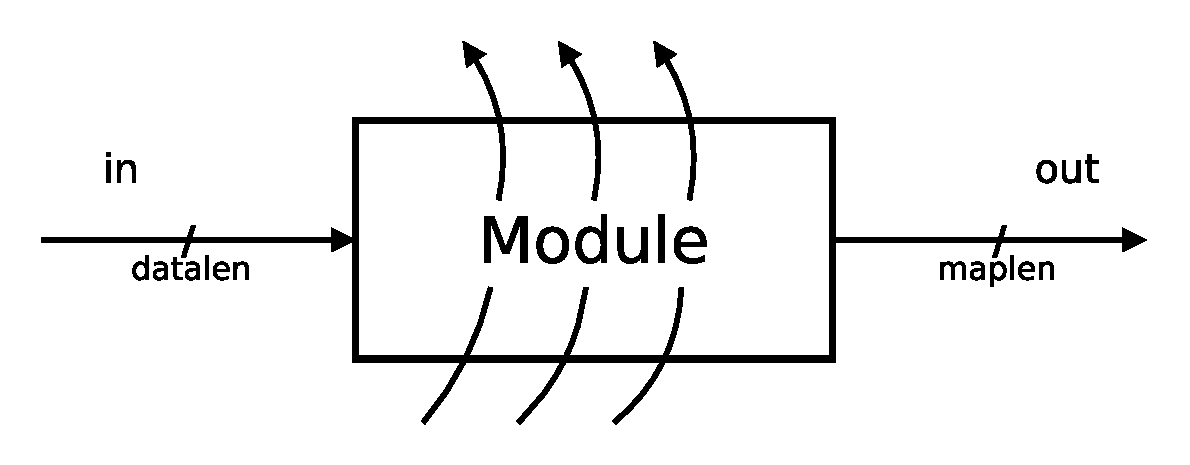
\includegraphics[scale=.5]{map}
%\vspace{-2ex}
\caption{Map Circuit Structure}
\label{fig-map}
\end{figure}

\end{document}

